\documentclass{article}

% if you need to pass options to natbib, use, e.g.:
% \PassOptionsToPackage{numbers, compress}{natbib}
% before loading nips_2018
\usepackage[numbers]{natbib}

% ready for submission
\usepackage{nips_2018}

% to compile a preprint version, e.g., for submission to arXiv, add
% add the [preprint] option:
% \usepackage[preprint]{nips_2018}

% to compile a camera-ready version, add the [final] option, e.g.:
% \usepackage[final]{nips_2018}

% to avoid loading the natbib package, add option nonatbib:
% \usepackage[nonatbib]{nips_2018}

\usepackage[utf8]{inputenc} % allow utf-8 input
\usepackage[T1]{fontenc}    % use 8-bit T1 fonts
\usepackage{hyperref}       % hyperlinks
\usepackage{url}            % simple URL typesetting
\usepackage{booktabs}       % professional-quality tables
\usepackage{amsfonts}       % greenboard math symbols
\usepackage{nicefrac}       % compact symbols for 1/2, etc.
\usepackage{microtype}      % microtypography

\usepackage[ruled, linesnumbered, noend]{algorithm2e}
\usepackage[para]{footmisc}
\usepackage[nosumlimits,tbtags]{amsmath}
% \usepackage{amsmath}
\usepackage{amsthm}
\usepackage{bm}
\usepackage{mathtools}
\usepackage{multirow}
\usepackage{nicefrac}
\usepackage{overpic}
\usepackage{subcaption}
\usepackage{tikz}
\usepackage{xcolor}

\usetikzlibrary{arrows,calc,positioning,shadows,shapes}


\usepackage{interval}
\intervalconfig{soft open fences}

\newtheorem{theorem}{Theorem}[section]
\newtheorem{corollary}{Corollary}[theorem]
\newtheorem{lemma}[theorem]{Lemma}
\newtheorem*{corollary1}{Corollary 4.1}
\newtheorem*{theorem1}{Theorem 4.2}
\newtheorem*{lemma1}{Lemma 4.3}

\usepackage{array}
\newcolumntype{L}[1]{>{\raggedright\let\newline\\\arraybackslash\hspace{0pt}}m{#1}}
\newcolumntype{C}[1]{>{\centering\let\newline\\\arraybackslash\hspace{0pt}}m{#1}}
\newcolumntype{R}[1]{>{\raggedleft\let\newline\\\arraybackslash\hspace{0pt}}m{#1}}

\newcommand{\DIF}{\mathrm{d}}
\newcommand{\OVEC}[1]{\bm{#1}} % vector
\newcommand{\SVEC}[1]{\check{\bm{#1}}}
\newcommand{\MAT}[1]{\mathbf{#1}} % matrix
\newcommand{\COL}[1]{\mathcal{#1}} % list, dict
\newcommand{\RSK}[1]{\mathcal{#1}} % loss, risk
\newcommand{\ERSK}[1]{\mathcal{#1}_{\rm{e}}} % loss, risk
\newcommand{\LOSS}[2]{\mathcal{#1}_{\rm{#2}}} % loss, risk
\newcommand{\UTIL}[1]{U(s,t,d)} % utility

\newcommand{\EXP}{\mathbb{E}} % expectation
\newcommand{\DTN}{\mathcal{L}_{\rm{D}}}

\newcommand{\CMNT}[1]{\colorbox{red!16}{\parbox{\dimexpr\linewidth-2\fboxsep}{\strut #1\strut}}}
\newsavebox\CBox\def\TBF#1{\sbox\CBox{#1}\resizebox{\wd\CBox}{\ht\CBox}{\textbf{#1}}}

\DeclareMathOperator{\COV}{Cov}
\DeclareMathOperator{\VAR}{Var}

\newcommand{\kddist}{\LOSS{\hat{D}}{}}
\newcommand{\kdganjs}{\LOSS{\tilde{D}}{}}
\newcommand{\kdgance}{\LOSS{\bar{D}}{}}
\newcommand{\kldiv}{\LOSS{L}{KL}}
\newcommand{\kdloss}{\LOSS{L}{KD}}
\newcommand{\kdganloss}{\LOSS{L}{KDGAN}}
\newcommand{\ganabbrobj}{\hat{U}}
\newcommand{\kdganabbrobj}{U}
\newcommand{\kdganfullobj}{U(s,t,d)}
\newcommand{\kdganmin}{\min_{s,t}}
\newcommand{\kdganmax}{\max_{d}}
\newcommand{\negloss}{\LOSS{L}{N}}
\newcommand{\posloss}{\LOSS{L}{P}}
\newcommand{\stddistloss}{\LOSS{L}{D}^{s}}
\newcommand{\tchdistloss}{\LOSS{L}{D}^{t}}
\newcommand{\stdgrad}{\nabla_{s}}
\newcommand{\stddisgrad}{\stdgrad\negloss}
\newcommand{\stdtchgrad}{\stdgrad\stddistloss}
\newcommand{\tchgrad}{\nabla_{t}}
\newcommand{\disgrad}{\nabla_{d}}

% probability distributions
% \newcommand{\pclf}{p_{\rm{m}}(\OVEC{y}|\OVEC{x})}
% \newcommand{\ppri}{p_{\rm{m}}^{\varrho}(\OVEC{x},\OVEC{y})}
\newcommand{\pclf}{p_{m}(\OVEC{y}|\OVEC{x})}
\newcommand{\ppri}{p_{m}^{\varrho}(\OVEC{x},\OVEC{y})}
% \newcommand{\abbrpdat}{p_{\rm{u}}}
% \newcommand{\fullpdat}{p_{\rm{u}}(\OVEC{y}|\OVEC{x})}
\newcommand{\abbrpdat}{p_{u}}
\newcommand{\fullpdat}{p_{u}(\OVEC{y}|\OVEC{x})}
% \newcommand{\abbrpstd}{p_{\rm{s}}}
% \newcommand{\abbrqstd}{q_{\rm{s}}}
% \newcommand{\fullpstd}[1]{p_{\rm{s}}(#1|\OVEC{x})}
% \newcommand{\fullqstd}[1]{q_{\rm{s}}(#1|\OVEC{x})}
\newcommand{\abbrpstd}{p_{s}}
\newcommand{\abbrqstd}{q_{s}}
\newcommand{\fullpstd}[1]{p_{s}(#1|\OVEC{x})}
\newcommand{\fullqstd}[1]{q_{s}(#1|\OVEC{x})}
% \newcommand{\abbrptch}{p_{\rm{t}}^{\varrho}}
% \newcommand{\abbrqtch}{q_{\rm{t}}^{\varrho}}
% \newcommand{\fullptch}[1]{p_{\rm{t}}^{\varrho}(#1|\OVEC{x})}
% \newcommand{\fullqtch}[1]{q_{\rm{t}}^{\varrho}(#1|\OVEC{x})}
\newcommand{\abbrptch}{p_{t}^{\varrho}}
\newcommand{\abbrqtch}{q_{t}^{\varrho}}
\newcommand{\fullptch}[1]{p_{t}^{\varrho}(#1|\OVEC{x})}
\newcommand{\fullqtch}[1]{q_{t}^{\varrho}(#1|\OVEC{x})}
% \newcommand{\abbrpdis}{p_{\rm{d}}^{\varrho}}
% \newcommand{\fullpdis}[1]{p_{\rm{d}}^{\varrho}(\OVEC{x},#1)}
\newcommand{\abbrpdis}{p_{d}^{\varrho}}
\newcommand{\fullpdis}[1]{p_{d}^{\varrho}(\OVEC{x},#1)}
% \newcommand{\abbrpcls}{p_{\rm{r}}}
% \newcommand{\fullpcls}{p_{\rm{r}}(\OVEC{y})}
\newcommand{\abbrpcls}{p_{r}}
\newcommand{\fullpcls}{p_{r}(\OVEC{y})}
% \newcommand{\abbrpmix}{p_{\rm{\alpha}}^{\varrho}}
% \newcommand{\fullpmix}{p_{\rm{\alpha}}^{\varrho}(\OVEC{y}|\OVEC{x})}
\newcommand{\abbrpmix}{p_{\alpha}^{\varrho}}
\newcommand{\fullpmix}{p_{\alpha}^{\varrho}(\OVEC{y}|\OVEC{x})}
% scoring function
\newcommand{\stdscore}{h(\OVEC{x},\OVEC{y})}
\newcommand{\tchscore}{g^{\varrho}(\OVEC{x},\OVEC{y})}
\newcommand{\disscore}{f^{\varrho}(\OVEC{x},\OVEC{y})}
% \newcommand{\priscore}[1]{s^{\varrho}_{\rm{#1}}(\OVEC{x},\OVEC{y})}
\newcommand{\priscore}[1]{s^{\varrho}_{#1}(\OVEC{x},\OVEC{y})}

\newcommand{\traindata}{\mathcal{D}}

\usepackage{colonequals}
\newcommand*{\LOGEQ}{\Leftrightarrow}

% default 
\setlength{\textfloatsep}{20.0pt plus 2.0pt minus 4.0pt}
\setlength{\floatsep}{12.0pt plus 2.0pt minus 2.0pt}
\setlength{\intextsep}{12.0pt plus 2.0pt minus 2.0pt}
% customized
\setlength{\textfloatsep}{15.0pt plus 2.0pt minus 4.0pt}
\setlength{\floatsep}{5.0pt plus 2.0pt minus 2.0pt}
\setlength{\intextsep}{10.0pt plus 2.0pt minus 2.0pt}

\title{KDGAN: A Unified Framework for Knowledge Distillation and Generative Adversarial Networks}

% The \author macro works with any number of authors. There are two
% commands used to separate the names and addresses of multiple
% authors: \And and \AND.
%
% Using \And between authors leaves it to LaTeX to determine where to
% break the lines. Using \AND forces a line break at that point. So,
% if LaTeX puts 3 of 4 authors names on the first line, and the last
% on the second line, try using \AND instead of \And before the third
% author name.

\author{
%   David S.~Hippocampus\thanks{Use footnote for providing further
%     information about author (webpage, alternative
%     address)---\emph{not} for acknowledging funding agencies.} \\
%   Department of Computer Science\\
%   Cranberry-Lemon University\\
%   Pittsburgh, PA 15213 \\
%   \texttt{hippo@cs.cranberry-lemon.edu} \\
  %% examples of more authors
  %% \And
  %% Coauthor \\
  %% Affiliation \\
  %% Address \\
  %% \texttt{email} \\
  %% \AND
  %% Coauthor \\
  %% Affiliation \\
  %% Address \\
  %% \texttt{email} \\
  %% \And
  %% Coauthor \\
  %% Affiliation \\
  %% Address \\
  %% \texttt{email} \\
  %% \And
  %% Coauthor \\
  %% Affiliation \\
  %% Address \\
  %% \texttt{email} \\
}

\begin{document}
% \nipsfinalcopy is no longer used

\maketitle


\begin{abstract}
Knowledge distillation (KD) enables a student model to learn from a pre-trained teacher.
Unfortunately, KD cannot theoretically guarantee the ideal equilibrium where the student perfectly fits the data distribution.
The ideal equilibrium can be guaranteed by a vanilla generative adversarial networks (GAN) where the student and teacher are learned via adversarial training.
However, the vanilla GAN requires massive training data and epochs to learn the student.
It is a challenge to design a single framework which guarantee the ideal equilibrium and accelerate the training with less data and epochs.
To address the challenge, we propose to power knowledge distillation with generative adversarial networks (KDGAN).
In KDGAN, we introduce a discriminator outside the student and teacher in a minimax game.
The discriminator trains the student to generate more realistic instances and approach the ideal equilibrium using an adversarial loss of the generated instances.
Meanwhile, the student is trained to generate more realistic instances with less data and epochs using a distillation loss of the outputs of the teacher.
To further accelerate the training, we reduce the variance of gradients with concrete distributions -- continuous relaxations for the student and teacher.
Experiments in the tasks of model compression and tag recommendation on various datasets show that KDGAN achieves significant performance gains over several baselines and requires less training data and epochs than the vanilla GAN.
\end{abstract}


\section{Introduction}

Knowledge distillation (KD) is one example of the machine-teaching-machine paradigm \cite{lopez2015unifying} where machines learn from other machines besides training instances \cite{fouad2013incorporating,sharmanska2013learning}.
In KD, a student model is trained to predict the true labels and \emph{soft labels}, i.e., class probabilities outputted by a pretrained teacher \cite{hinton2015distilling}.
% The student is deployed to perform inference while the teacher is available only during training.
% The teacher is expected to reach a better equilibrium than the student if optimized only with training data.
% Thus, the teacher can regularize the student to generalize better with the soft labels which reveal helpful information about each training examples and impose much more constraint on the student's parameters.
% Building such a teacher normally involves resources that are accessible for model training and are not available at testing.
% For example, Hinton et al. \cite{hinton2015distilling} build a teacher with large learning capacity using extensive computing power easily available at training.
% Another example is that Lopez-Paz et al. \cite{lopez2015unifying} build a teacher with better performance using privileged information, i.e., features available only at training.
% Although KD has several advantages such as fast convergence rate and being data efficient, it does not provide a theoretical guarantee of the ideal equilibrium in which the student perfectly fits the data distribution.
The student can reach a better equilibrium with less training data and epochs as the soft labels reveal helpful information for each training instance and impose much constraint on updating the student.
To obtain such soft labels, the teacher is normally trained with resources that are only accessible for model training.
For example, Hinton et al. \cite{hinton2015distilling} train a teacher with a large learning capacity using extensive computing power and Lopez-Paz et al. \cite{lopez2015unifying} train a teacher with better performance using privileged information about training instances.
However, KD does not provide a theoretical guarantee of the ideal equilibrium in which the student exactly replicates the data distribution.
This is because the pretrained teacher is not perfect and thus the soft labels are noisy to some extent.
In the face of such noisy labels, the student learns to fit some incorrect instances made by the teacher, which results in a deviation from the ideal equilibrium.

The ideal equilibrium can be guaranteed by a vanilla generative adversarial network (GAN) which can be also considered an example of the machine-teaching-machine paradigm.
The vanilla GAN corresponds to a minimax game in which the student acts as a generator and the teacher servers as a discriminator \cite{wang2017irgan}.
The minimax game can be formulated as an optimization that minimizes a distance measure between the data distribution and the student distribution.
Since the distance measure is minimized iff the student distribution is exactly the same as the data distribution, the equilibrium of the vanilla GAN is ideal.
One problem with the vanilla GAN is that the training requires a large number of training instances and often delves into slow convergence and unstable behavior \cite{feizi2017understanding}.
A reason for the problem is that as the discriminator reaches the ideal equilibrium, the gradients from the discriminator on training the generator usually vanish or explode \cite{arjovsky2017towards}.
The vanishing gradients prevent the student from being further improved while the exploding gradients make the training slow and unstable.
Hence, it is a challenge to train the student towards fitting the data distribution in the ideal equilibrium with less training instances and epochs.

To address this challenge, we propose a unified framework KDGAN (knowledge distillation boosted with generative adversarial networks).
In KDGAN, we define a student generator (referred to as a student), a teacher generator (referred to as a teacher), and a discriminator.
The student and teacher aim to model the data distribution and fool the discriminator by generating pseudo labels that look like the true labels.
In contrast, the discriminator justifies the quality of the pseudo labels and guides the student and teacher in generating more realistic labels via adversarial training.
The adversarial training can be formulated as an optimization that minimizes the distance between the data distribution and a linear combination of the student distribution and teacher distribution.
At the same time, the student and teacher try to reach an agreement and generate the same pseudo labels for a training instance.
To achieve this, we minimize the distance between the student distribution and teacher distribution via knowledge distillation.
The equilibrium of KDGAN is ideal because the student will perfectly match the data distribution when the two distances are set to the minimum.

Different from the vanilla GAN, the student in KDGAN also receives gradients for the soft labels from the teacher.
The gradients for the soft labels are usually non-zero with low variance, which can tackle the problem of vanishing and exploding gradients and accelerate the training in the vanilla GAN.
To further accelerate the training, we reduce the gradient variance by smoothing the pseudo labels with a concrete distribution, a continuous relaxation for the student (or teacher).
The concrete distribution contains a temperature parameter which controls the smoothness of the pseudo labels, which is scheduled from a high temperature to a low temperature in experiments.

To sum up, our main contributions include:
% (1) We propose a novel KDGAN framework which can achieve the ideal equilibrium guaranteed by GAN and the fast convergence brought by KD simultaneously.
% We leverage the concrete distributions to prevent the slow adversarial training in GAN from damping the advantage of fast convergence in KD.
% (2) We show that KDGAN can achieve significant performance gain over strong baselines in two real-world applications including image tag recommendation and deep model compression.
% We further show that the KDGAN training requires less training examples and epochs than the vanilla GAN. 
(1) We propose a novel KDGAN framework to integrate the strengths of KD and GAN.
In the integration, we leverage the concrete distribution to keep GAN from damping the advantage of KD.
(2) We show that KDGAN outperforms the state-of-the-art methods in the tasks of deep model compression and image tag recommendation.
Furthermore, we show that KDGAN requires less labeled instances and training epochs than the vanilla GAN.


\section{Related Work}

% The machine-teaching-machine paradigm \cite{lopez2015unifying} has gained considerable attention recently, such as adversarial learning \cite{chongxuan2017triple} and knowledge distillation \cite{lopez2015unifying}.

\TBF{Generative Adversarial Networks (GAN)} are initially proposed to generate continuous data with a generator through an adversarial game against a discriminator \cite{goodfellow2014generative}.
GANs have only recently been introduced to generate discrete data, since unlike continuous data, discrete data makes it difficult to update the generator by passing gradients backwards.
For example, sequence GAN (SeqGAN) \cite{yu2017seqgan} models token sequence generation as a stochastic policy in reinforcement learning and adopts Monte Carlo search to update the generator.
% Another example is the minimax game for information retrieval (IRGAN) \cite{wang2017irgan} proposed to generate relevant documents (or items) from a candidate pool given a query (or a user).
Different from these GANs with two players, Li et al. propose triple GANs with three players called Triple-GAN \cite{chongxuan2017triple}.
Our KDGAN also consists of three players including two generators and a discriminator, but differs from Triple-GAN in that:
(1) Both generators in KDGAN model a conditional distribution of labels given features.
However, the generators in Triple-GAN model a conditional distribution of labels given features and a conditional distribution of features given labels respectively.
(2) The samples from the generators in KDGAN are all discrete data.
In contrast, the samples from the generators in Triple-GAN include both discrete data and continuous data.
These differences lead to different objective functions and training algorithms, e.g., we can use the Gumbel-Max trick \cite{gumbelstatistical,maddison2014sampling} to sample from both generators in KDGAN.


\TBF{Knowledge Distillation (KD)} aims to transfer the knowledge of a powerful teacher network into a lightweight student network with fewer parameters.
For example, Ba and Caruana \cite{ba2014deep} propose to train a shallow student model to mimic a deep teacher model by matching logits before the last softmax layer.
Hinton et al. \cite{hinton2015distilling} generalize this work and use the soft labels (i.e., the class probabilities produced by the teacher) to train the student.
Sau and Balasubramanian \cite{sau2016deep} propose to add random perturbation to the soft labels, which simulates learning from multiple teacher models.
Lopez-Paz et al. \cite{lopez2015unifying} unify KD \cite{hinton2015distilling} and privileged information \cite{vapnik2015learning} as generalized distillation in which a teacher is pre-trained with privileged information and then a student is trained to fit the soft labels from the teacher.
One of the differences between KD and our work is that during the training of the student, the teacher in KD is fixed but the teacher in our work can still be improved.

We explore the idea of integrating the strengths of KD and GANs.
A similar idea has been studied in \cite{xu2017learning} where a discriminator is introduced to encourage a student in generating data that is not distinguishable from the data generated by a teacher.
This is different from our work in which a discriminator is introduced to encourage the student in generating data that is not distinguishable from the real data.
Furthermore, the objective functions proposed by Xu et al. for the student and the discriminator are different \cite{xu2017learning}.
On the contrary, the objective functions for the student and the discriminator are the same in our work which brings a theoretical advantage (detailed in Section \ref{sec:kdgan formulation}).


\section{Preliminaries}

\begin{figure}[tbp]
\centering
\setlength{\abovecaptionskip}{4pt plus 0pt minus 0pt}
\tikzset{
diagonal fill/.style 2 args={fill=#2, path picture={
\fill[#1, sharp corners] (path picture bounding box.south west) -|
                         (path picture bounding box.north east) -- cycle;}},
reversed diagonal fill/.style 2 args={fill=#2, path picture={
\fill[#1, sharp corners] (path picture bounding box.north west) |- 
                         (path picture bounding box.south east) -- cycle;}}
}
\tikzstyle{student} = [rectangle, draw, text centered,
  minimum height=0.80cm, minimum width=2.00cm,
  fill=red!8!white,
]
\tikzstyle{teacher} = [rectangle, draw, text centered,
  minimum height=0.80cm, minimum width=2.00cm,
  fill=blue!8!white,
]
\tikzstyle{generator} = [diagonal fill={blue!8!white}{red!8!white}, draw, text centered,
  minimum height=0.80cm, minimum width=2.00cm,
]
\tikzstyle{data} = []
% \begin{minipage}{1.00\textwidth}
\begin{tikzpicture}
% help line
% \draw[help lines] (0.50,0.00) grid (14.50,3.50);

% node
\node [rectangle] at (0.80,0.60) {$\OVEC{x}$};
\node [rectangle] at (0.80,1.00) {$\varrho$};
\node [rectangle] at (0.80,2.36) {$\OVEC{x}$};

% line
\draw [->,blue,thick,dashed] (0.96,0.60) -- (1.80,0.60);
\draw [->,blue,thick,dashed] (0.96,1.00) -- (1.80,1.00);
\draw [->,red,thick,dotted] (0.96,2.36) -- (1.80,2.36);

% line
\draw [->,blue,thick,dashed] (2.20,2.40) -- (2.20,1.20);
\draw [->,blue,thick,dashed] (2.20,0.40) -- (2.20,0.20) -- (3.80,0.20);
\draw [->,red,thick,dotted] (3.40,1.20) -- (3.40,2.16);
\draw [->,red,thick,dotted] (3.40,2.96) -- (3.40,3.16) -- (3.80,3.16);

% distillation losses
\node [rectangle] at (5.36,0.20) {\small{$\DTN(\fullpstd{\OVEC{y}},\fullptch{\OVEC{y}})$}};
\node [rectangle] at (5.36,3.16) {\small{$\DTN(\fullptch{\OVEC{y}},\fullpstd{\OVEC{y}})$}};
% teacher
\node [teacher] (tch) at (2.80,0.80) {\small{Teacher}};
% student
\node [student] (std) at (2.80,2.56) {\small{Student}};
% student soft labels
\node [rectangle,fill=white] at (1.60,1.68) {\small{$\OVEC{y}_{s}\sim\fullpstd{\OVEC{y}}$}};
% teacher soft labels
\node [rectangle,fill=white] at (4.00,1.68) {\small{$\OVEC{y}_{t}\sim\fullptch{\OVEC{y}}$}};
% the true labels
\node [rectangle] at (6.40,1.68) {\small{$\OVEC{y}\sim\fullpdat$}};

% discriminator label line
\draw [->,green,thick] (3.80,1.08) -- (7.72,1.08);
\draw [->,green,thick] (7.32,1.68) -- (7.72,1.68);
\draw [->,green,thick] (3.80,2.28) -- (7.72,2.28);
% discriminator feature line
% \draw [->,green,thick] (7.32,0.48) -- (7.72,0.48) -- (8.72,0.94);
% \draw [->,green,thick] (7.32,2.88) -- (7.72,2.88) -- (8.72,2.42);
\draw [->,green,thick] (7.32,0.48) -- (7.72,0.80);
\draw [->,green,thick] (7.32,2.88) -- (7.72,2.56);

% teacher pseudo labels
\node [rectangle,fill=white] at (5.76,1.08) {\small{$\SVEC{y}_{t}\sim\fullqtch{\OVEC{y}}$}};
% student pseudo labels
\node [rectangle,fill=white] at (5.76,2.28) {\small{$\SVEC{y}_{s}\sim\fullqstd{\OVEC{y}}$}};

% discriminator
% \node [discriminator] (dis) at (9.80,2.20) {\small{Discriminator}};
\draw[fill=green!8] (7.72,0.80) -- (7.72,2.56) -- (9.72,2.28) -- (9.72,1.08) -- cycle;
\node at (8.72,1.68) {\small{Discriminator}};
% discriminator input node
\node at (7.16,0.48) {\small{$\OVEC{x}$}};
\node at (7.16,2.88) {\small{$\varrho$}};

% line
\draw [->,green,thick] (9.72,1.16) -- (10.12,1.16);
\draw [->,green,thick] (9.72,1.68) -- (10.12,1.68);
\draw [->,green,thick] (9.72,2.20) -- (10.12,2.20);

\node at (12.36,1.12) {\small{$\LOSS{L}{N}=\EXP_{\OVEC{y}\sim\abbrptch}[\log(1-\fullpdis{\OVEC{y}})]$}};
\node at (12.00,1.68) {\small{$\LOSS{L}{P}=\EXP_{\OVEC{y}\sim\abbrpdat}[\log\fullpdis{\OVEC{y}}]$}};
\node at (12.36,2.24) {\small{$\LOSS{L}{N}=\EXP_{\OVEC{y}\sim\abbrpstd}[\log(1-\fullpdis{\OVEC{y}})]$}};

\end{tikzpicture}
% \end{minipage}
\caption{
An illustration of KDGAN with privileged provision $\varrho$ available only at training.
The KDGAN framework consists of a student $\fullpstd{\OVEC{y}}$, a teacher $\fullptch{\OVEC{y}}$, and a discriminator  $\fullpdis{\OVEC{y}}$ which are colored in red, blue, and green respectively with $\fullqstd{\OVEC{y}}$ and $\fullqtch{\OVEC{y}}$ denoting the continuous relaxations for the student and the teacher, $\LOSS{L}{N}$ and $\LOSS{L}{P}$ denoting adversarial losses of negative labels and positive labels for the discriminator, and $\DTN$ denoting a distillation loss.
}
\label{fig:kdgan}
\end{figure}

In this paper, we study the multi-label classification problem \cite{hinton2015distilling,lopez2015unifying,vapnik2015learning}, where we have privileged provision $\varrho$ that represents additional resources accessible for model training besides the training instances $\traindata=\{(\OVEC{x}_{1},\OVEC{y}_{1}),...,(\OVEC{x}_{n},\OVEC{y}_{n})\}$.
Privileged provision can be for example additional information about training instances \cite{vapnik2015learning} (often called privileged information) and extra computing power for model training \cite{ba2014deep,hinton2015distilling,sau2016deep} (compared with limited computing power such as on mobile devices).
Since privileged provision is not available at testing, the goal is to fit the data distribution $\fullpdat$ with a lightweight classifier $\pclf$ that does not require privileged provision for effective inference.

To achieve the goal, there are two broad classes of methods, KD-based and GAN-based, which learn such a classifier $\pclf$ from a model $\ppri$ that leverages privileged provision $\varrho$.
We propose KDGAN according to our insight that advantages and disadvantages of KD-based and GAN-based methods are complementary to one another.
On one hand, KD-based methods \cite{ba2014deep} view $\ppri$ as a teacher which outputs soft labels and train $\pclf$ to maximize the probability of predicting the soft labels.
KD-based methods cannot guarantee the ideal equilibrium where $\pclf=\fullpdat$, but have an advantage that a small number of training instances and epochs are generally sufficient.
On the other hand, GAN-based methods \cite{wang2017irgan} view $\ppri$ as a discriminator which judges whether a feature-label pair is from the real data, and train $\pclf$ to maximize the discriminator's probability of making incorrect judgments.
GAN-based methods have an advantage that the ideal equilibrium is guaranteed in theory, but a large number of training instances and epochs are required.
It is challenging to achieve the advantages of both classes of methods simultaneously in a single framework.


\section{KDGAN Framework}

We propose the KDGAN framework to train a lightweight classifier with less training examples and epochs.
An overview of KDGAN is presented in Figure \ref{fig:kdgan}.
The KDGAN framework consists of three player, a student $\fullpstd{\OVEC{y}}$, a teacher $\fullptch{\OVEC{y}}$, and a discriminator $\fullpdis{\OVEC{y}}$.
The student does not use privileged provision and is our target lightweight classifier.
The teacher and discriminator can both access privileged provision and are available only at training.
The three players are combined in a minimax game where the student and teacher minimize the discriminator's objective.
Given $\OVEC{x}$ as input, the student and teacher output categorical distributions over labels.
The categorical distributions are relaxed with concrete distributions used to sample pseudo labels.
The student and teacher minimize the discriminator's probability of rejecting the pseudo labels as the real labels, whereas the discriminator maximizes the probability of correctly distinguishing between the real labels and pseudo labels.
Besides, the teacher produces soft labels from its categorical distribution for the student to learn.
To make KDGAN more general, we also enable the teacher to learn from the student's soft labels.
Since the concrete distributions keep the relative order regarding the relevancy of labels as the categorical distributions, the mutual learning between the student and teacher can be viewed as minimizing the probability of generating different pseudo labels for a training instance.
% The rationale behind such a three-player framework is based on our observations that: (1) The introduction of a discriminator into KD helps to achieve a better equilibrium because as long as the discriminator succeeds in distinguishing the pseudo labels from the true labels, it can provide feedback for the student and the teacher to make them generate more realistic labels.
% (2) The introduction of a teacher into GAN helps to accelerate the adversarial training because the discriminator and the student can receive more training signals with the training data generated by the teacher (i.e., pseudo labels for the discriminator and soft labels for the student).

\subsection{KDGAN Formulation} \label{sec:kdgan formulation}

% We formulate KDGAN as a training framework that minimizes (1) the distance (with a proper measure) between a student distribution and a teacher distribution, and (2) the distance between the data distribution and a linear combination of the student distribution and the teacher distribution.
We formulate KDGAN as a three-player minimax game with a value function $\kdganfullobj$ defined as
% \begin{small}
\begin{equation} \label{equ:objective function}
\hspace*{-0.01cm}
\begin{aligned}
\kdganmin
\kdganmax
\kdganfullobj
=
% \EXP_{\fullpdat}[\log\fullpstd{\OVEC{y}}]
\EXP_{\OVEC{y}\sim\abbrpdat}[\log\fullpdis{\OVEC{y}}]
&
+
% \alpha\EXP_{\fullpstd{\OVEC{y}}}[\log(1-\fullpdis{\OVEC{y}})]
\alpha\EXP_{\OVEC{y}\sim\abbrpstd}[\log(1-\fullpdis{\OVEC{y}})]
\\
+
% (1-\alpha)\EXP_{\OVEC{y}\sim\fullptch{\OVEC{y}}}[\log(1-\fullpdis{\OVEC{y}})]
(1-\alpha)
\EXP_{\OVEC{y}\sim\abbrptch}[\log(1-\fullpdis{\OVEC{y}})]
+
\beta
&
\stddistloss(\fullpstd{\OVEC{y}},\fullptch{\OVEC{y}})
% \beta\DTN(\fullpstd{\OVEC{y}},p_{\rm{s}}(\OVEC{y}|\OVEC{x}\mathrlap{))}
+
\gamma
\tchdistloss(\fullptch{\OVEC{y}},\fullpstd{\OVEC{y}})
% \gamma\DTN(\fullptch{\OVEC{y}},p_{\rm{t}}^{\varrho}(\OVEC{y}|\OVEC{x}\mathrlap{))}
\text{,}
\\
\end{aligned}
\end{equation}%
% \end{small}
% where $\alpha\in\interval{0}{1}$ balances the relative importance of the discriminator competing against the teacher and student and $\beta\in\interval[open left, open right]{0}{+\infty}$ together with $\gamma\in\interval[open left, open right]{0}{+\infty}$ controls the strength of knowledge distillation between the student and teacher.
where $\alpha\in\interval{0}{1}$, $\beta\in\interval[open left, open right]{0}{+\infty}$, and $\gamma\in\interval[open left, open right]{0}{+\infty}$ are hyper-parameters.
On the right-hand side of Equation \ref{equ:objective function}, $\stddistloss$ and $\tchdistloss$ are referred to as the \emph{distillation losses} while the other three terms are referred to as the \emph{adversarial losses}.
Distillation losses $\stddistloss$ and $\tchdistloss$ influence the student and teacher respectively, which are often defined as the L2 loss on logits \cite{ba2014deep} or the cross entropy on distributions \cite{hinton2015distilling}.
% , e.g., $\DTN(\fullpstd{\OVEC{y}},\fullptch{\OVEC{y}})$ can be defined as:
% \begin{small}
% \begin{equation} \label{equ:l2 norm distillation loss}
% \begin{aligned}
% \DTN(\fullpstd{\OVEC{y}},\fullptch{\OVEC{y}})
% =
% {\textstyle\frac{1}{2}}\EXP_{\OVEC{y}\sim\fullpcls}
% [||\log\fullptch{\OVEC{y}}-\log\fullpstd{\OVEC{y}}||^{2}]
% \end{aligned}
% \end{equation}
% \end{small}%
% Here, $\fullpcls$ is the true distribution over labels.
% Distillation losses can also be defined by the cross entropy \cite{hinton2015distilling}, e.g., $\DTN(\fullpstd{\OVEC{y}},\fullptch{\OVEC{y}})$ can be defined as:
% \begin{small}
% \begin{equation} \label{equ:cross entropy distillation loss}
% \begin{aligned}
% \DTN(\fullpstd{\OVEC{y}},\fullptch{\OVEC{y}})
% =
% \EXP_{\OVEC{y}\sim\text{softmax}(\log\fullptch{\OVEC{y}}/\omega)}
% [-\log\text{softmax}({\textstyle\frac{\log\fullpstd{\OVEC{y}}}{\omega}})]
% \text{,}
% \end{aligned}
% \end{equation}
% \end{small}%
% where $\omega \in \interval[open left, open right]{0}{+\infty}$ is a temperature parameter.
% The discriminator estimates the probability of a given label $\OVEC{y}$ is from the data distribution or not, which is defined as:
% \begin{small}
% \begin{equation}
% \fullpdis{\OVEC{y}}
% =
% \text{sigmoid}(\disscore)
% =
% {\textstyle\frac{\exp(\disscore)}{1+\exp(\disscore)}}
% \text{,}
% \end{equation}
% \end{small}%
% where $\disscore$ is a scoring function.
The student and teacher compute a class probability $\OVEC{y}$ given an example $\OVEC{x}$ while the discriminator computes the probability that a feature-label pair $(\OVEC{x}, \OVEC{y})$ is from the real data,
% \begin{small}
\begin{equation}
\fullpstd{\OVEC{y}}
=
% \frac{\exp(h_{c}(\OVEC{x},\OVEC{y}))}{\sum_{\OVEC{y}}\exp(h_{c}(\OVEC{x},\OVEC{y}))}
\text{softmax}(\stdscore)
\text{, } \ 
\fullptch{\OVEC{y}}
=
% \frac{\exp(g_{t}(\OVEC{x},\OVEC{y},\OVEC{z}))}{\sum_{\OVEC{y}}\exp(g_{t}(\OVEC{x},\OVEC{y},\OVEC{z}))}
\text{softmax}(\tchscore)
\text{, } \ 
\fullpdis{\OVEC{y}}
=
\text{sigmoid}(\disscore)
\end{equation}
% \end{small}%
where $\stdscore$, $\tchscore$, and $\disscore$ are scoring functions for the student, teacher, and discriminator.
The scoring functions can be implemented in various ways, e.g., $\stdscore$ is implemented as a two-layer perceptron \cite{lecun1998gradient}, which will be discussed in the next section.
% We leave the discussions on the scoring functions to the next section when we discuss specific classification problems.

\TBF{Theoretical Analysis}.
We prove that KDGAN can guarantee the ideal equilibrium where the student perfectly models the data distribution.
We refer to $\fullpmix=\alpha\fullpstd{\OVEC{y}}+(1-\alpha)\fullptch{\OVEC{y}}$ as the \emph{mixture distribution}.
Note that both student and teacher generate pseudo labels, we find that sampling from the student and teacher is equivalent to sampling from the mixture distribution because 
% \begin{small}
\begin{equation}
\begin{aligned}
\alpha\EXP_{\OVEC{y}\sim\abbrpstd}
&
[\log(1-\fullpdis{\OVEC{y}})]
+
(1-\alpha)\EXP_{\OVEC{y}\sim\abbrptch}[\log(1-\fullpdis{\OVEC{y}})]
\\
&=
\alpha{\textstyle\sum}_{\OVEC{y}}\,
\fullpstd{\OVEC{y}}\log(1-\fullpdis{\OVEC{y}})
+
(1-\alpha){\textstyle\sum}_{\OVEC{y}}\,
\fullptch{\OVEC{y}}\log(1-\fullpdis{\OVEC{y}})
\\
&=
{\textstyle\sum}_{\OVEC{y}}\,
\big(\alpha\fullpstd{\OVEC{y}}+(1-\alpha)\fullptch{\OVEC{y}}\big)
\log(1-\fullpdis{\OVEC{y}})
\\
&=
\EXP_{\OVEC{y}\sim\abbrpmix}[\log(1-\fullpdis{\OVEC{y}})]
\text{.}
\end{aligned}
\end{equation}
% \end{small}%
Because of this, the adversarial losses correspond to a two-player game with a value function,
% \begin{small}
\begin{equation}
\begin{aligned}
\min_{\alpha}
\max_{d}
\EXP_{\OVEC{y}\sim\abbrpdat}[\log\fullpdis{\OVEC{y}}]
+
\EXP_{\OVEC{y}\sim\abbrpmix}[\log(1-\fullpdis{\OVEC{y}})]
\text{,}
\end{aligned}
\end{equation}%
% \end{small}%
where the mixture distribution is the generator.
According to \cite{goodfellow2014generative,wang2017irgan}, the global minimum of such two-player game is achieved iff the mixture distribution (or the generator) perfectly fit the data distribution.
Thus, the minimization of the adversarial losses imposes a constraint that $\fullpmix=\fullpdat$ at the KDGAN equilibrium.
Besides, the minimization of the distillation losses imposes another constraint that the student distribution and teacher distribution are exactly the same $\fullpstd{\OVEC{y}}=\fullptch{\OVEC{y}}$ at the KDGAN equilibrium.
The KDGAN equilibrium is achieved iff the two constraints are simultaneously satisfied, where the student perfectly match the data distribution.

Formally, we provide some theoretical results about KDGAN.
We first show that the optimal discriminator balances between the data distribution and the mixture distribution, as stated below.
\begin{corollary1} \label{cor:optimal discriminator}
For any fixed student and teacher, the objective function $\kdganfullobj$ is maximized if and only if the discriminator $\fullpdis{\OVEC{y}}=\nicefrac{\fullpdat}{(\fullpdat+\fullpmix)}$.
\end{corollary1}%
Further, we show that the equilibrium of the minimax game is achieved iff both the student and teacher are exactly the same as the data distribution, which is summarized as follows.
\begin{theorem1} \label{thm:ideal equilibrium}
The equilibrium of the minimax game $\kdganmin\kdganmax\kdganfullobj$ is achieved if and only if $\fullpstd{\OVEC{y}}=\fullptch{\OVEC{y}}=\fullpdat$. At that point, $\kdganfullobj$ reaches the value $-\log 4$.
\end{theorem1}%

The proofs of the theoretical results are deferred to Appendix \ref{app:theory}.

\subsection{KDGAN Training} \label{sec:kdgan training}

\begin{algorithm}[tbp]
\small
\DontPrintSemicolon
\KwIn{ Training data $\traindata=\{(\OVEC{x}_{1},\OVEC{y}_{1}),...,(\OVEC{x}_{n},\OVEC{y}_{n})\}$ with privileged provision $\varrho$. }

Pretrain a student $\fullpstd{\OVEC{y}}$, a teacher $\fullptch{\OVEC{y}}$, and a discriminator $\fullpdis{\OVEC{y}}$ with the training data $\traindata$. \\

\For{ number of training epochs } {

\For{ number of training steps for the discriminator } {
Compute the continuous relaxations $\fullqstd{\OVEC{y}}$ and $\fullqtch{\OVEC{y}}$ for the student and the teacher respectively. \\
Use $\fullpdat$, $\fullqstd{\OVEC{y}}$, and $\fullqtch{\OVEC{y}}$ to sample labels $\{\OVEC{y}_{1},...,\OVEC{y}_{k}\}$, $\{\SVEC{y}^{1}_{s},...,\SVEC{y}^{k}_{s}\}$, and $\{\SVEC{y}^{1}_{t},...,\SVEC{y}^{k}_{t}\}$. \\
Update the discriminator by ascending along its gradient \\
% \begin{small}
$
\frac{1}{k}
\sum_{i=1}^{k}
\big(
\nabla_{d}
\log\fullpdis{\OVEC{y}_{i}}
+
\alpha\nabla_{d}\log(1-\fullpdis{\SVEC{y}^{i}_{s}})
+
(1-\alpha)\nabla_{d}\log(1-\fullpdis{\SVEC{y}^{i}_{t}})
\big)
\text{.}
$
% \end{small}
\\
}

\For{ number of training steps for the teacher } {
Compute the continuous relaxation $\fullqtch{\OVEC{y}}$ for the teacher and use it to sample labels $\{\SVEC{y}^{1}_{t},...,\SVEC{y}^{k}_{t}\}$. \\
Update the teacher by descending along its gradient \\
% \begin{small}
$
\frac{1}{k}
\sum_{i=1}^{k}
(1-\alpha)
\nabla_{t}\log\fullqtch{\OVEC{y}^{i}_{t}}
\log(1-\fullpdis{\SVEC{y}^{i}_{t}})
+
\gamma
\nabla_{t}
\tchdistloss(\fullptch{\OVEC{y}},\fullpstd{\OVEC{y}})
\text{.}
$
% \end{small}
\\
}

\For{ number of training steps for the student } {
Compute the continuous relaxation $\fullqstd{\OVEC{y}}$ for the student and use it to sample labels $\{\SVEC{y}^{1}_{s},...,\SVEC{y}^{k}_{s}\}$. \\
Update the student by descending along its gradient \\
% \begin{small}
$
\frac{1}{k}
\sum_{i=1}^{k}
\alpha
\nabla_{s}\log\fullqstd{\OVEC{y}^{i}_{s}}
\log(1-\fullpdis{\SVEC{y}^{i}_{s}})
+
\beta
\nabla_{s}
\stddistloss(\fullpstd{\OVEC{y}},\fullptch{\OVEC{y}})
\text{.}
$
% \end{small}
\\
}
}

\caption{ Minibatch stochastic gradient descent training of KDGAN. }
\label{alg:kdgan}
\end{algorithm}

Integrating KD into GAN reduces the gradient variance compared with the vanilla GAN, which can accelerate the training of the student.
We show that the high variance of a random variable can be reduced with a low-variance random variance (refer to Appendix \ref{app:theory} for proofs), as summarized below.
\begin{lemma1}
Let $X$ and $Y$ be two random variables that satisfy a condition $\VAR(X)\leq\VAR(Y)$.
Then for all $\lambda\in\interval{0}{1}$, we have $\VAR(Z)\leq\VAR(Y)$ where $Z = \lambda X+ (1-\lambda) Y$.
\end{lemma1}
The student in the vanilla GAN only receives the gradients $\stddisgrad$ from the discriminator, whereas the student in the proposed KDGAN also receives the gradients $\stdtchgrad$ from the teacher, $\stdgrad\kdganabbrobj=\lambda\stddisgrad+(1-\lambda)\stdtchgrad$ where $\lambda\in\interval{0}{1}$.
Consistent with previous observations \cite{hinton2015distilling,sau2016deep}, we find that $\stdtchgrad$ usually have small variance and have smaller variance than $\stddisgrad$ $\VAR(\stdtchgrad)\leq\VAR(\stddisgrad)$, which satisfy the condition of Lemma 4.3.
According to Lemma 4.3, the gradient variance for the student in KDGAN, $\VAR(\stdgrad\kdganabbrobj)$, is lower than the vanilla GAN, $\VAR(\stdgrad\kdganabbrobj)$,
% \begin{small}
\begin{equation}
\begin{aligned}
\hspace*{-0.04cm}
\VAR(\stdtchgrad)\leq\VAR(\stddisgrad)
\text{,}
\;
\stdgrad\kdganabbrobj=\lambda\stddisgrad+(1-\lambda)\stdtchgrad
\Rightarrow
\VAR(\stdgrad\kdganabbrobj)\leq\VAR(\stddisgrad)
\text{.}
\end{aligned}
\end{equation}%
% \end{small}%
However, the gradient variance can be high as the gradients from the adversarial losses usually have high variance \cite{chongxuan2017triple,yu2017seqgan}.
Most methods for reducing this gradient variance rely on a control variate \cite{mnih2016variational,wang2017irgan}.
Even with such a control variate, the gradients can still have high variance because the pseudo labels used to estimate the gradients are discrete variances.

To further reduce the gradient variance, we leverage a continuous relaxation of discrete variables.
As the discrete variances are sampled from a categorical distribution, we use a concrete distribution, a continuous relaxation of categorical variables, to relax the categorical distribution.
The concrete distribution for the student is defined as
% \begin{small}
\begin{equation} \label{equ:student concrete distribution}
\begin{aligned}
\fullqstd{\OVEC{y}}
=
% \text{softmax}({\textstyle\frac{\log\fullpstd{\OVEC{y}}+\OVEC{g}}{\tau}})
% \text{softmax}(\frac{\log\fullpstd{\OVEC{y}}+\OVEC{g}}{\tau})
\text{softmax}(\nicefrac{(\log\fullpstd{\OVEC{y}}+\OVEC{g})}{\tau})
\text{, } \quad
\OVEC{g}=-\log(-\log(\OVEC{u}))
\text{, } \quad
\OVEC{u}\sim\text{uniform}\interval[open left, open right]{0}{1}
\text{,}
\end{aligned}
\end{equation}%
% \end{small}%
where $\tau\in\interval[open left, open right]{0}{+\infty}$ is a temperature.
With a high temperature, the pseudo labels sampled from the concrete distribution are smooth and the variance of the gradients $\nicefrac{\partial\abbrqstd}{\partial\abbrpstd}$ is small, which results in low-variance gradient estimates for the student.
However, the concrete distribution with a high temperature becomes less exact approximation to the categorical distribution, which results in biased gradient estimates.
We tune the temperature to achieve a good balance between bias and variance.
We find that a reasonable schedule for the temperature is to start with a high temperature and then exponentially decay to a small temperature.
We leave the exploration of the optimal schedule to future work.

The overall logic of the KDGAN framework is summarized in Algorithm \ref{alg:kdgan}.
The student, the teacher, and the discriminator can be pre-trained separately and then the three players are trained alternatively in a number of training epochs.
The detailed derivation of the gradients is provided in Appendix \ref{app:gradient}.

% \TBF{Rationale of the KDGAN Training}.
% The proposed KDGAN training introduces two mechanisms to accelerate and stabilize the optimization by reducing the variance of the gradients.
% The first mechanism is by introducing knowledge distillation between the student and the teacher.
% The second mechanism is by relaxing the categorical distributions ($\abbrpstd$ and $\abbrptch$) with the concrete distributions ($\abbrqstd$ and $\abbrqtch$).


\section{Experiments}

\begin{table} [tbp]
\small
\centering
\setlength{\abovecaptionskip}{6pt plus 0pt minus 0pt}
\setlength\tabcolsep{5.0pt}
% \begin{tabular}{l|ccc|ccc}
\begin{tabular}{l|C{1.66cm}C{1.66cm}C{1.66cm}|C{1.66cm}C{1.66cm}C{1.66cm}}
\toprule
\multirow{2}{*}{Method} & \multicolumn{3}{c|}{ MNIST } & \multicolumn{3}{c}{ CIFAR-10 } \\
\cmidrule(rl){2-4}
\cmidrule(rl){5-7}
& $n=100$ & $n=1000$ & $n=10000$ & $n=500$ & $n=5000$ & $n=50000$ \\
\midrule
% Student & 54.94 $\pm$ 0.13 & 86.57 $\pm$ 0.17 & 97.13 $\pm$ 0.09 & 45.29 $\pm$ 0.20 & 71.11 $\pm$ 0.14 & 80.34 $\pm$ 0.12 \\
GAN & 64.90 $\pm$ 0.31 & 93.60 $\pm$ 0.22 & 98.95 $\pm$ 0.19 & 46.29 $\pm$ 0.32 & 76.11 $\pm$ 0.24 & 85.34 $\pm$ 0.27 \\
DistnMdl & 68.34 $\pm$ 0.06 & 93.97 $\pm$ 0.11 & 98.79 $\pm$ 0.11 & 50.92 $\pm$ 0.18 & 76.59 $\pm$ 0.15 & 83.32 $\pm$ 0.08 \\
NoisyTch & 66.53 $\pm$ 0.18 & 93.45 $\pm$ 0.08 & 98.58 $\pm$ 0.07 & 50.18 $\pm$ 0.28 & 75.42 $\pm$ 0.19 & 82.99 $\pm$ 0.12 \\
MimicLog & 67.35 $\pm$ 0.15 & 93.78 $\pm$ 0.13 & 98.65 $\pm$ 0.05 & 51.74 $\pm$ 0.23 & 75.66 $\pm$ 0.17 & 84.33 $\pm$ 0.10 \\
\midrule
KDGAN & \TBF{77.95} $\pm$ 0.05 & \TBF{96.42} $\pm$ 0.05 & \TBF{99.25} $\pm$ 0.02 & \TBF{57.56} $\pm$ 0.13 & \TBF{79.36} $\pm$ 0.04 & \TBF{86.50} $\pm$ 0.04 \\ 
\bottomrule
\end{tabular}
\caption{ Accuracy averaged by 10 runs for model compression ($n$ is the number of training images). }
\label{tab:deep model compression overall}
\end{table}

\begin{figure}[tbp]
\centering
\setlength{\abovecaptionskip}{4pt plus 0pt minus 0pt}
\begin{subfigure}{0.33\textwidth}
 \centering
 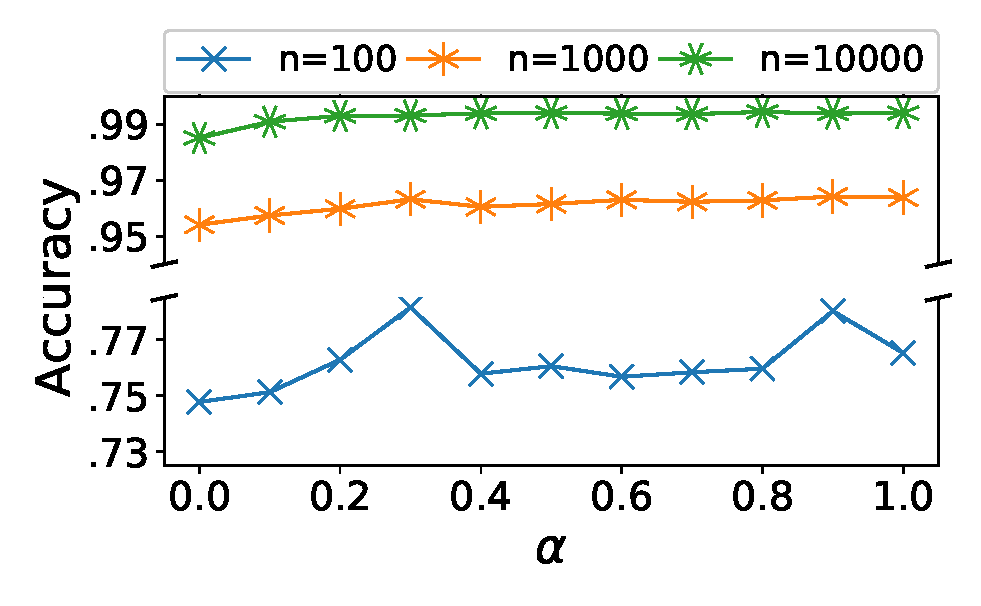
\includegraphics[width=1.00\linewidth]{mdlcompr_mnist_alpha.eps}
\end{subfigure}
\hspace*{-0.4em} % \hfill
\begin{subfigure}{0.33\textwidth}
 \centering
 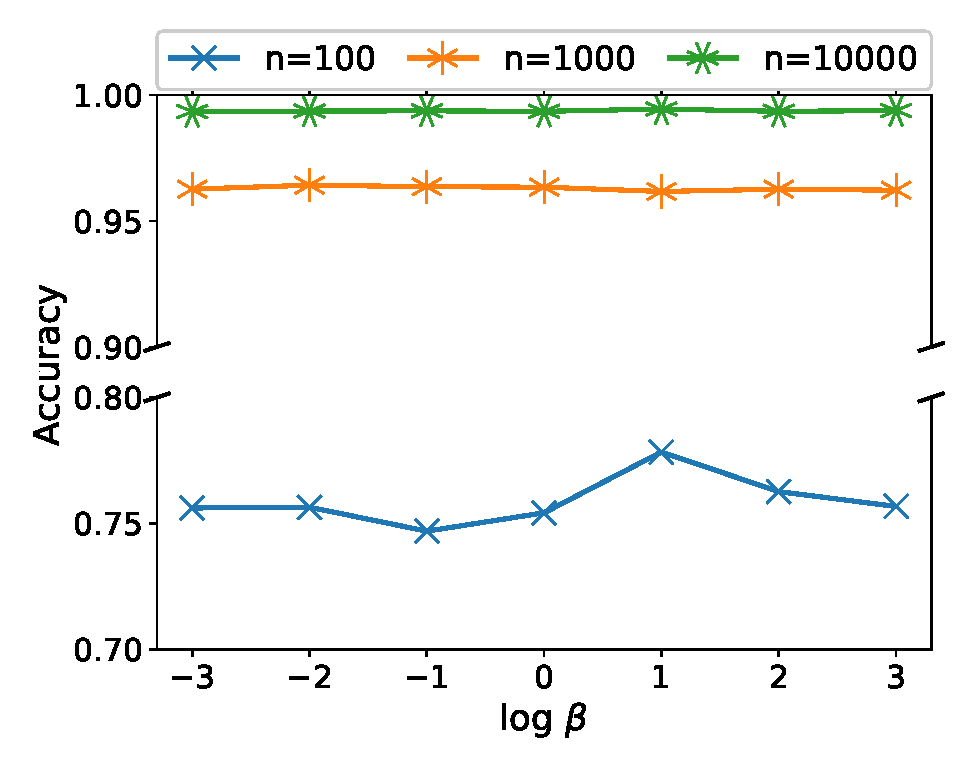
\includegraphics[width=1.00\linewidth]{mdlcompr_mnist_beta.eps}
\end{subfigure}
\hspace*{-0.4em} % \hfill
\begin{subfigure}{0.33\textwidth}
 \centering
 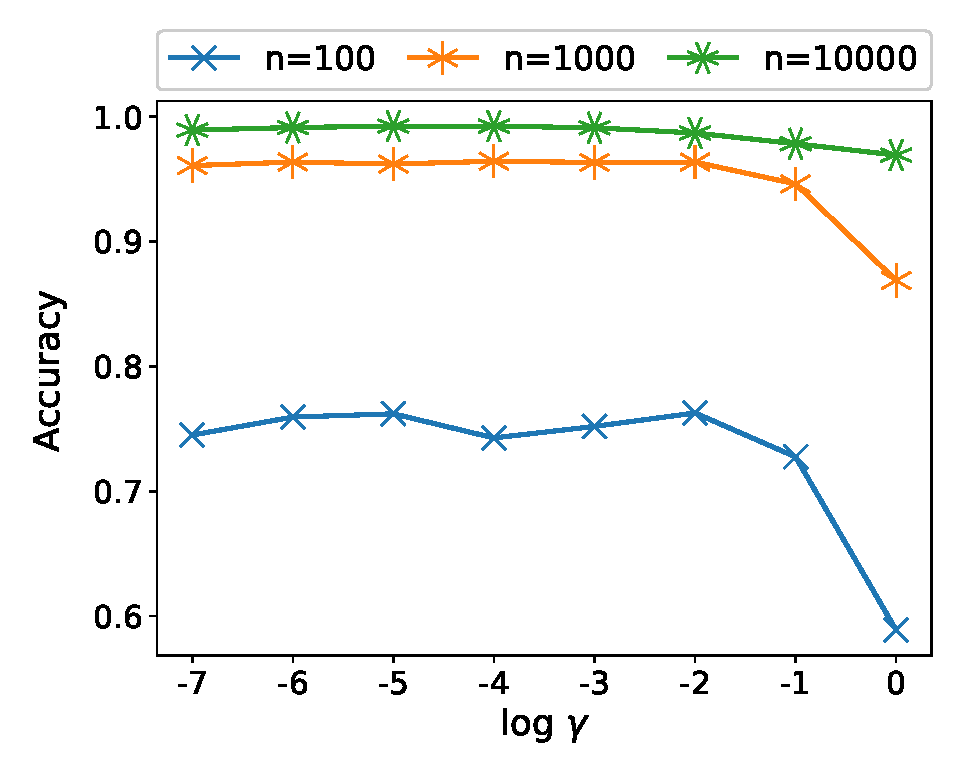
\includegraphics[width=1.00\linewidth]{mdlcompr_mnist_gamma.eps}
\end{subfigure}
\caption{ Effects of hype-parameters on the MNIST dataset in the task of deep model compression. }
\label{fig:deep model compression tuning}
\end{figure}

We apply KDGAN to the problems of image tag recommendation and deep model compression where privileged provision is prominent.
Generally, KDGAN can be applied to a wide range of classification problems with privileged provision.
For simplicity, we implement the teacher and discriminator using the same scoring function but with different parameter sets:
% \begin{small}
\begin{equation}
\tchscore
=
\priscore{t}
\quad
\text{and}
\quad
\disscore
=
\priscore{d}
\end{equation}%
% \end{small}%
We first test the vanilla GAN and proposed KDGAN within the problem of deep model compression and then KDGAN is further investigated in the problem of image tag recommendation.

\subsection{Deep Model Compression} \label{sec:deep model compression}

The task of deep model compression is to reduce the storage and runtime complexity of deep models and improve the deployability of such models, for example, on mobile devices.
Extensive computing power available at training is considered privileged provision in this task.

\TBF{Experiment Setup}.
We make use of the widely used MNIST \cite{lecun1998gradient} and CIFAR-10 \cite{krizhevsky2009learning} datasets.
The MNIST dataset consists of 10 labels and 60,000 gray images (50,000 for training and 10,000 for testing).
Following \cite{sau2016deep}, we do not preprocess the images on MNIST.
The CIFAR-10 dataset contains 10 labels and 60,000 colored images (50,000 for training and 10,000 for testing).
We preprocess the images by subtracting per-pixel mean and augment the training set by mirrored images.

We implement $\stdscore$ and $\priscore{}$ as a MLP \cite{lecun1998gradient} and a LeNet \cite{lecun1998gradient} on MNIST, and implement $\stdscore$ and $\priscore{}$ as a LeNet \cite{lecun1998gradient} and a ResNet \cite{he2016deep} on CIFAR-10 (detailed in Appendix \ref{app:architecture}).
We compare KDGAN with the vanilla GAN and KD-based methods including DistnMdl \cite{hinton2015distilling}, MimicLog \cite{ba2014deep}, and NoisyTch \cite{sau2016deep} in terms of accuracy.
To see how the performance of different methods vary against the size of training data, we experiment with different numbers of training images.

\TBF{Results and Discussions}.
The overall performances of the various methods are summarized in Table \ref{tab:deep model compression overall}.
The results show that KDGAN as an integration of KD and GAN brings a consistent performance improvement over the KD-based methods and vanilla GAN.
Compared with KD-based methods where the performance of the student is upper bounded by the pretrained teacher, the student in KDGAN outperforms the pretrained teacher on MNIST.
One possible reason is that the student, teacher, and discriminator are simultaneously trained in an adversarial way within KDGAN.
The discriminator pushes the teacher to generate more realistic labels and thus improves the teacher's performance.
This raises the upper bound of the student's performance, which makes it have the potential to outperform the pretrained teacher.
Compared with the vanilla GAN, KDGAN requires less labeled instances for training, which can be observed from the fact that KDGAN achieves a larger performance gain in the vases where we have less training instances.
This is because in KDGAN, the soft labels produced by the student and teacher generally have high entropy and provide much information about each training instance.
The soft labels can be viewed as additional training data to learn the student, which reduces the number of training instance and epochs required for training.
To further study the convergence rate, we compare the learning curves of the student in the proposed KDGAN and vanilla GAN.
The results are presented in Figure \ref{fig:learning curves}(a).
We can observe that the KDGAN training can accelerate and stabilize the learning process of the student.
This can be explained by that the teacher can provide non-zero gradients with low variance by the soft labels and the discriminator can provide more smooth gradients by sampling from the relaxation distributions at training.
% Moreover, we can see that the proposed KDGAN shows an advantage in the low-data regime: KDGAN has a significant lager performance gain over other methods in the cases where we have less labeled training examples.

We also investigate the performance of KDGAN against hyper-parameters $\alpha$, $\beta$, and $\gamma$.
The results are presented in Figure \ref{fig:deep model compression tuning}, note that the log scale of the x axis for Figures \ref{fig:deep model compression tuning}(b) and \ref{fig:deep model compression tuning}(c).
We can see that $\alpha$ and $\beta$ have a relatively small effect on the performance, which suggests that KDGAN is a stable and robust framework.
However, a large value of $\gamma$ can cause the performance to deteriorate greatly.
This is because the soft labels produced by the student model contain more noisy information than those produced by the teacher model.
Emphasizing too much on the student model distilling its knowledge into the teacher model will have a negative effect on the teacher model, which in turn hurts the performance of the student model.

\subsection{Image Tag Recommendation} \label{sec:image tag recommendation}


\begin{table} [tbp]
\small
\centering
\setlength{\abovecaptionskip}{6pt plus 0pt minus 0pt}
\setlength\tabcolsep{4.5pt}
% \begin{tabular}{l|cccccc|cccccc}
\begin{tabular}{l|C{0.72cm}C{0.72cm}C{0.72cm}C{0.72cm}C{0.72cm}C{0.72cm}|C{0.72cm}C{0.72cm}C{0.72cm}C{0.72cm}C{0.72cm}C{0.72cm}}
\toprule
\multirow{2}{*}{Method} & \multicolumn{6}{c|}{ Popular Labels } & \multicolumn{6}{c}{ Random Labels } \\
\cmidrule(rl){2-7}
\cmidrule(rl){8-13}
& P@3 & P@5 & F@3 & F@5 & MAP & MRR & P@3 & P@5 & F@3 & F@5 & MAP & MRR \\
\midrule
TagFeat & .2560 & .1752 & .2871 & .1999 & .6417 & .6503 & .2002 & .1420 & .2195 & .1495 & .5149 & .5309 \\
TagProp & .2420 & .1636 & .2811 & .1949 & .6177 & .6270 & .1883 & .1372 & .1810 & .1252 & .4512 & .4636 \\
KnnVote & .2320 & .1680 & .2339 & .1633 & .5755 & .5852 & .1623 & .1198 & .1575 & .1088 & .3970 & .4092 \\
RelExmp & .2720 & .1800 & .3324 & .2295 & .7015 & .7122 & .2228 & .1378 & .2427 & .1669 & .5205 & .5331  \\
\midrule
KDGAN & \TBF{.3047} & \TBF{.1968} & \TBF{.3678} & \TBF{.2526} & \TBF{.7787} & \TBF{.7905} & \TBF{.2572} & \TBF{.1666} & \TBF{.2946} & \TBF{.2009} & \TBF{.6302} & \TBF{.6452} \\
\bottomrule
\end{tabular}
\caption{ Performance of various methods on the YFCC100M dataset for image tag recommendation.  }
\label{tab:image tag recommendation overall}
\end{table}

\begin{figure}[tbp]
\centering
\setlength{\abovecaptionskip}{4pt plus 0pt minus 0pt}
\begin{subfigure}{.33\textwidth}
 \centering
 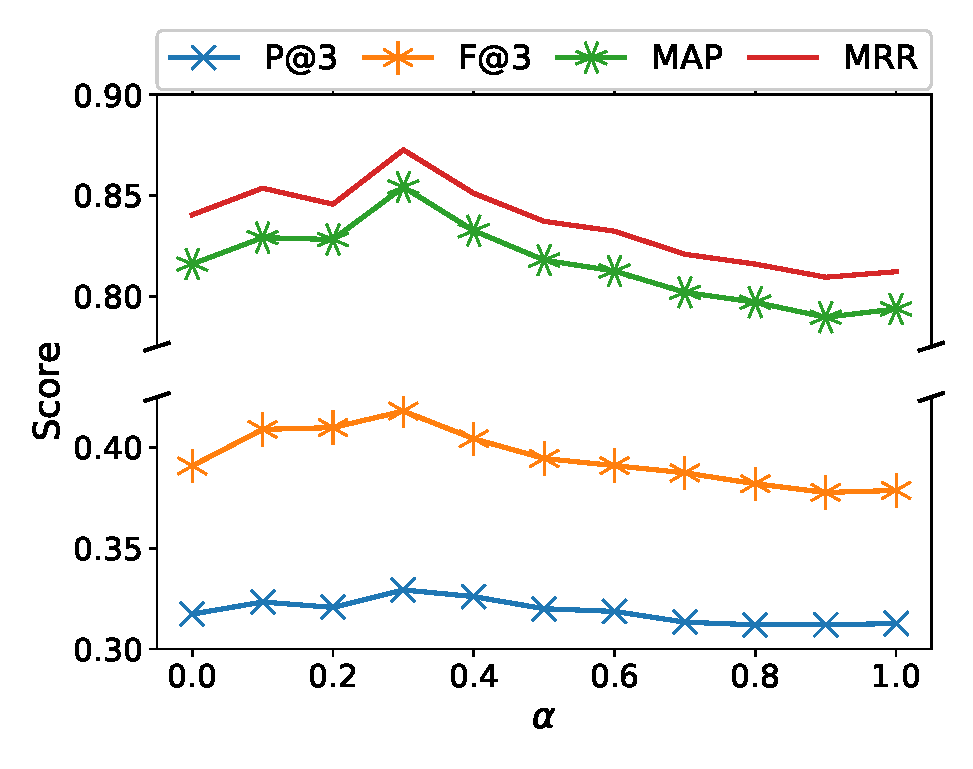
\includegraphics[width=1\linewidth]{tagrecom_yfcc10k_alpha.eps}
\end{subfigure}
\hspace*{-0.4em} % \hfill
\begin{subfigure}{.33\textwidth}
 \centering
 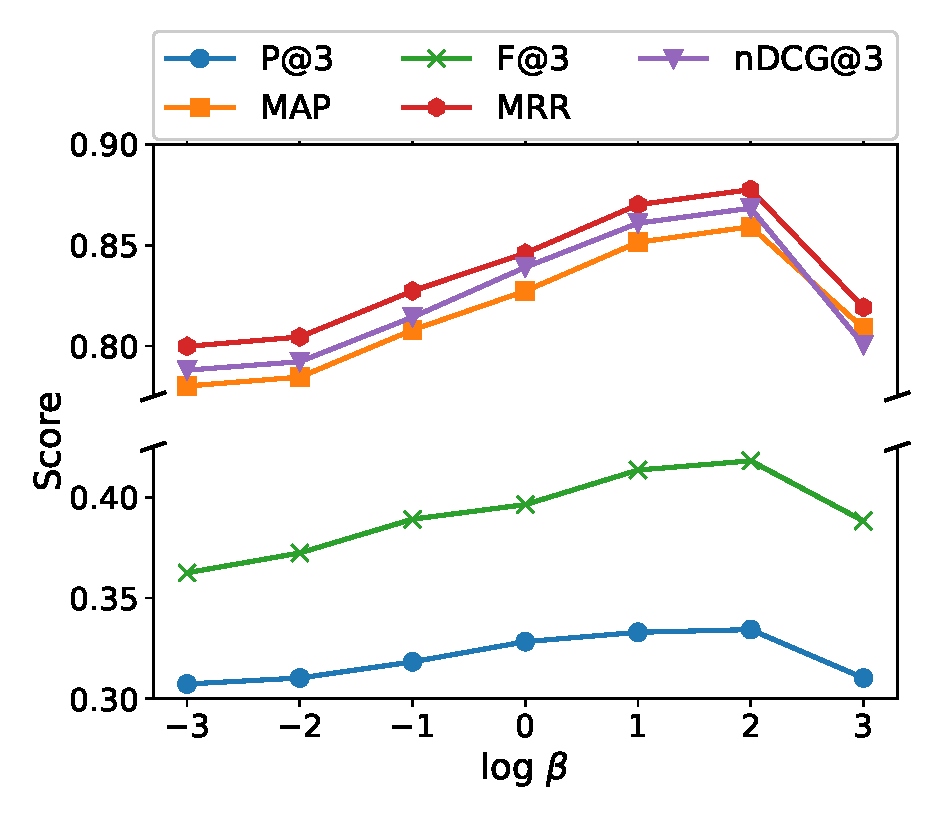
\includegraphics[width=1\linewidth]{tagrecom_yfcc10k_beta.eps}
\end{subfigure}
\hspace*{-0.4em} % \hfill
\begin{subfigure}{.33\textwidth}
 \centering
 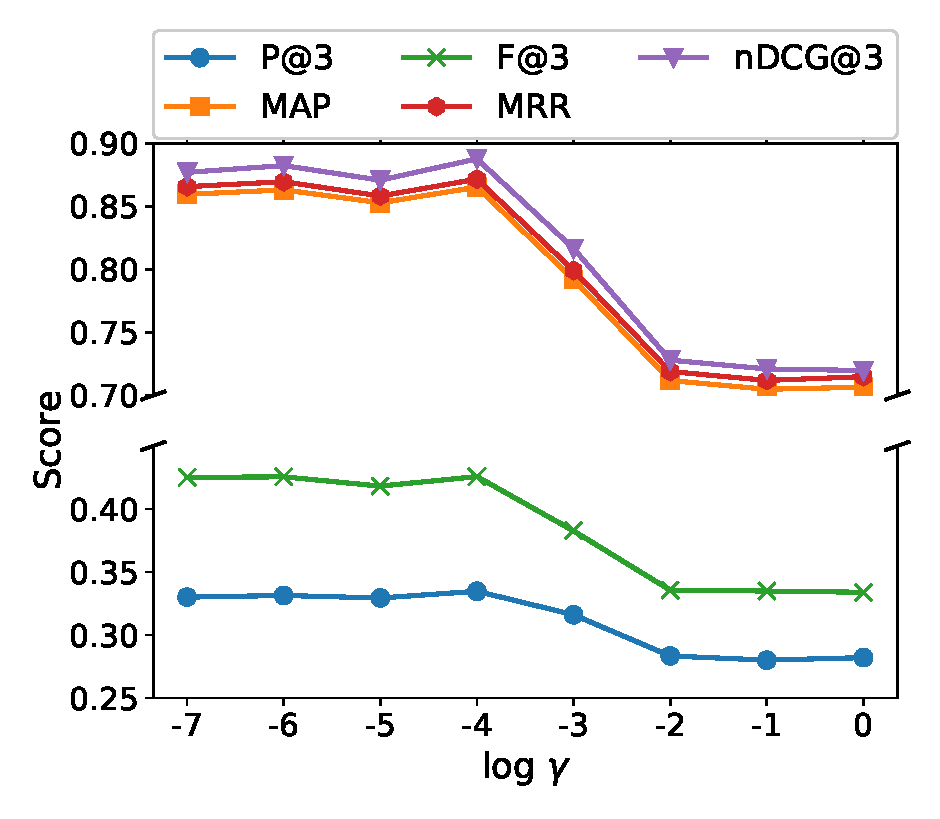
\includegraphics[width=1\linewidth]{tagrecom_yfcc10k_gamma.eps}
\end{subfigure}
\caption{ Effects of hype-parameters on the YFCC100M dataset in the task of image tag recommendation. }
\label{fig:image tag recommendation tuning}
\end{figure}

Image tag recommendation is to recommend relevant tags (or labels) after a user uploads an image to image-hosting websites such as Instagram\footnote{\url{https://www.instagram.com/}} or Flickr\footnote{\url{https://www.flickr.com/}}.
% For example, if a user uploads an image of a cat playing with a dog, we could recommend relevant tags such as ``cute kitten'', ``lovely pet'', ``brave dog'' etc.
It is common that additional text such as image titles and descriptions is provided during uploading the image.
Since text entering is not convenient especially on mobile devices, we aim to make recommendations after a user uploading an image before entering any text for better user experience.
Hence, we consider the additional text as privileged information in the task of image tag recommendation.


\TBF{Experiment Setup}.
We conduct experiments on the Yahoo Flickr Creative Commons 100 Million (YFCC100M) dataset \cite{thomee2016yfcc100m}.
To simulate the case where additional texts about images are available only at training, we randomly sample 20,000 images with additional text as the training set and another 2,000 images as the test set.
We create two YFCC100M subsets with different characteristics: one subset is annotated with the 200 most popular labels while the other is annotated with 200 randomly sampled labels.

Following existing work \cite{antol2015vqa}, we use a VGGNet \cite{simonyan2014very} pre-trained on ImageNet \cite{deng2009imagenet} to extract image features and a LSTM \cite{hochreiter1997long} with pre-trained word embeddings \cite{mikolov2013distributed} to learn text features.
We implement $\stdscore$ as a MLP with image features as inputs and $\priscore{}$ as a MLP with the element-wise product of image and text features as inputs.
The network architectures are detailed in Appendix \ref{app:architecture}.

In the experiment, we compare the student in KDGAN with KnnVote \cite{makadia2010baselines}, TagProp \cite{guillaumin2009tagprop}, TagFeat \cite{chen2012tag}, and RelExmp \cite{li2013classifying}.
We evaluate all algorithms by precision (P@N), F-score (F@N), mean average precision (MAP), and mean reciprocal ranking (MRR).

\TBF{Results and Discussions}.
Table \ref{tab:image tag recommendation overall} summarizes the results.
We can see that KDGAN achieves significant improvements over other methods across all the evaluation measures.
Although the student in KDGAN does not explicitly learn to model the semantic similarity between two tags like what RelExmp does, it still works consistently better than RelExmp.
A possible explanation is that the soft labels used to train the student contain a rich similarity structure over tags, which cannot be modeled well by any pairwise similarity between tags which is used by RelExmp.
For example, the soft labels for an image tagged with volleyball may have a probability of 10$^{-2}$ being tagged with basketball, 10$^{-4}$ of being tagged with baseball, and 10$^{-8}$ with dragonfly, which indicates that volleyball, basketball and baseball are more similar than the tag dragonfly.

We compare the learning curves of the proposed KDGAN and vanilla GAN.
The results are presented in Figure \ref{fig:learning curves}(b), which shows that the KDGAN training is much faster and more stable than the GAN training.
We also study the effect of hyper-parameters $\alpha$, $\beta$, and $\gamma$ in the task of image tag recommendation and present the results in Figure \ref{fig:image tag recommendation tuning}.
We can see that the results are consistent with our observations for deep model compression.

\section{Conclusion}

\begin{figure}[tbp]
\centering
\setlength{\abovecaptionskip}{4pt plus 0pt minus 0pt}
\begin{subfigure}{0.49\textwidth}
 \centering
 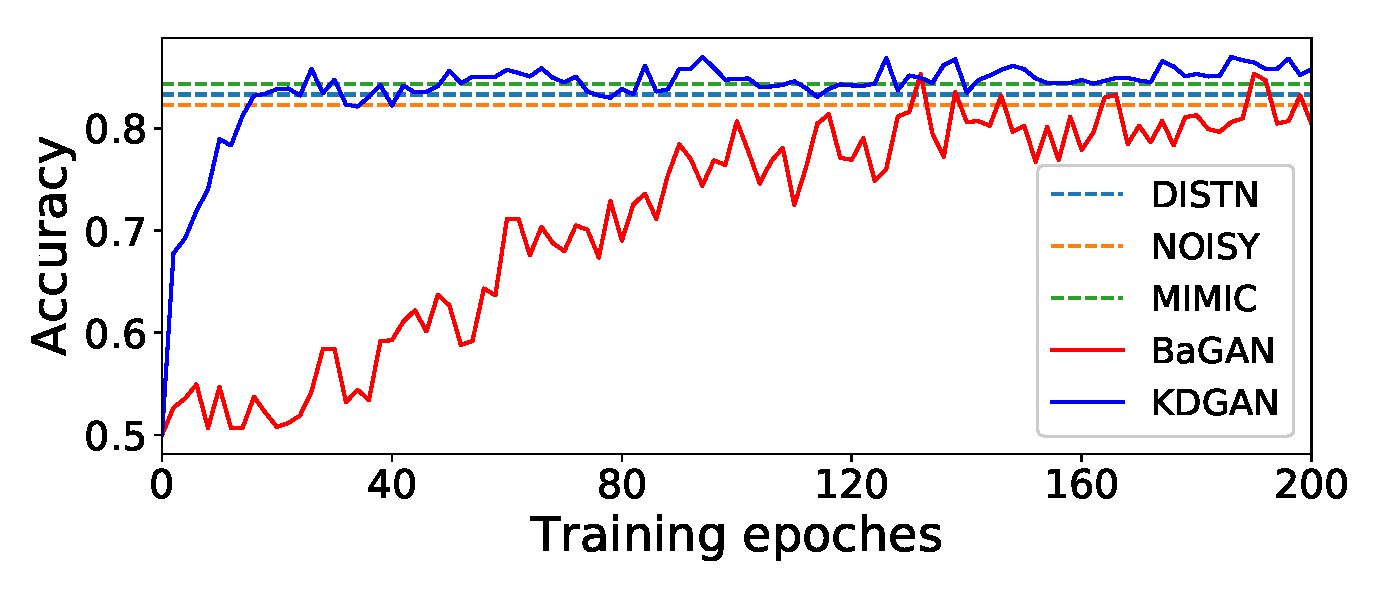
\includegraphics[width=1.00\linewidth]{mdlcompr_mnist_cr.eps}
  \caption{ Deep model compression. }
\end{subfigure}
\begin{subfigure}{0.49\textwidth}
 \centering
 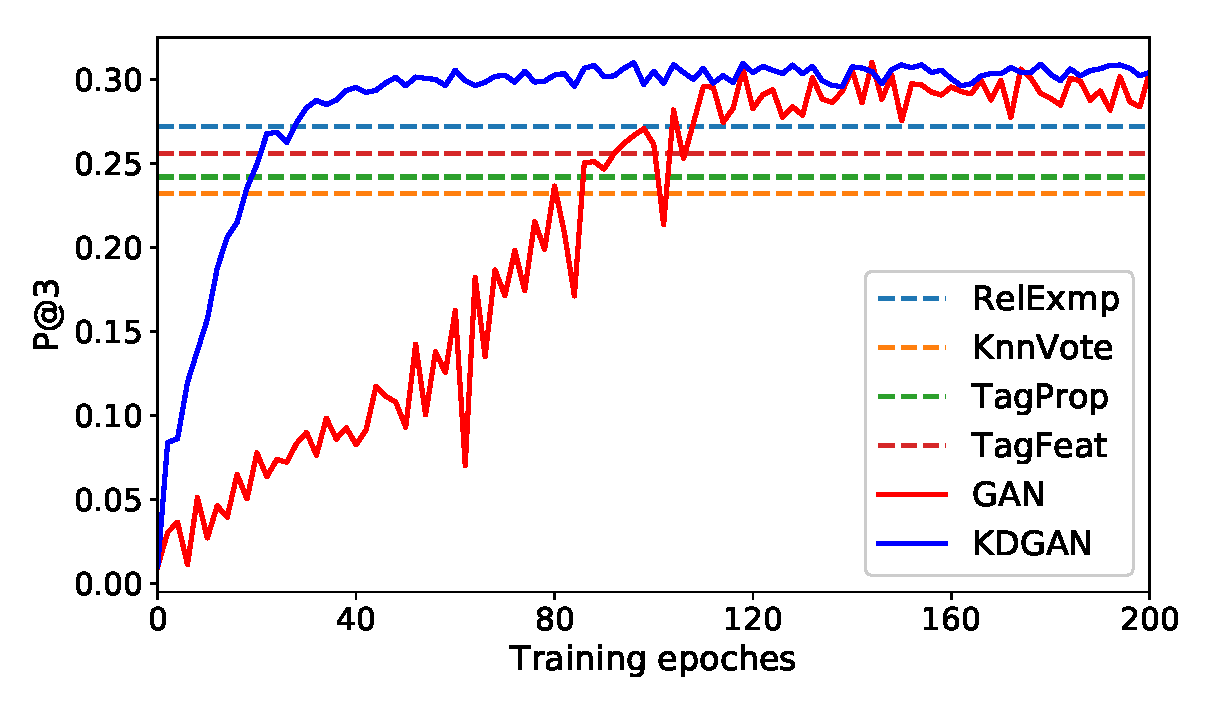
\includegraphics[width=1.00\linewidth]{tagrecom_yfcc10k_cr.eps}
  \caption{ Image tag recommendation. }
\end{subfigure}
\caption{ Learning curves of the proposed KDGAN and a vanilla GAN. }
\label{fig:learning curves}
\end{figure}

We proposed a game theory-based KDGAN framework to perform the learning using privileged provision, in which a student model, a teacher model, and a discriminative model are combined to play a minimax game.
Powered by carefully designed objective functions and optimization techniques, the student model in KDGAN can perfectly fit the underlying data distribution at a fast rate, which addresses the problem of limited performance gain in knowledge distillation and alleviates the problem of slow convergence in adversarial learning.
We applied KDGAN to image tag recommendation and deep model compression, two real-world applications in which privileged provision is available at training stage.
Our experimental results showed that KDGAN outperformed several state-of-the-art methods by a large margin (e.g., as much as 12.02\% on P@3 in image tag recommendation).
In the meantime, the training process of the student model was shown to be much faster and more stable than a straightforward application of adversarial learning to knowledge distillation.


% \clearpage
{
\scriptsize
% \bibliographystyle{unsrtnat}
\bibliographystyle{abbrvnat}
\bibliography{nips_2018}
}


\appendix


\section{Theoretical Analysis} \label{app:theory}

We theoretically analyze the global equilibrium of KDGAN in this section.
First we show that the optimal discriminator balances between the underlying data distribution and the mixture distribution defined by a student and a teacher, as stated in Lemma.
\begin{lemma1}
Given any student and teacher, the optimal discriminator is given by:
\begin{small}
\begin{equation*}
\fullpdis{\OVEC{y}}
=
\frac{\fullpdat}{\fullpdat+\fullpmix}
\end{equation*}%
\end{small}%
Here, $\fullpdat$ is the data distribution and $\fullpmix=\alpha\fullpstd{\OVEC{y}}+(1-\alpha)\fullptch{\OVEC{y}}$.
\end{lemma1}
 
\begin{proof}
The discriminator aims to maximize the objective function of the minimax game.
According to the definition of the expected value, the objective function can be rewritten as:
\begin{small}
\begin{equation*}
\begin{aligned}
\max_{d}
&
\,
\UTIL{}
\\
=
&
\,
% \max_{d}
% \big(
\EXP_{\OVEC{y}\sim\abbrpdat}[\log\fullpdis{\OVEC{y}}]
+
\alpha\EXP_{\OVEC{y}\sim\abbrpstd}[\log(1-\fullpdis{\OVEC{y}})]
+
(1-\alpha)\EXP_{\OVEC{y}\sim\abbrptch}[\log(1-\fullpdis{\OVEC{y}})]
% \big)
\\
=
&
\,
% \max_{d}
% \big(
\EXP_{\OVEC{y}\sim\abbrpdat}[\log\fullpdis{\OVEC{y}}]
+
\alpha\sum_{\mathclap{\OVEC{y}\in\COL{Y}}}
\fullpstd{\OVEC{y}}\log(1-\fullpdis{\OVEC{y}})
+
(1-\alpha)\sum_{\mathclap{\OVEC{y}\in\COL{Y}}}
\fullptch{\OVEC{y}}\log(1-\fullpdis{\OVEC{y}})
% \big)
\\
=
&
\,
% \max_{d}
% \big(
\EXP_{\OVEC{y}\sim\abbrpdat}[\log\fullpdis{\OVEC{y}}]
+
\sum_{\OVEC{y}\in\COL{Y}}
(\alpha\fullpstd{\OVEC{y}}+(1-\alpha)\fullptch{\OVEC{y}})\log(1-\fullpdis{\OVEC{y}}))
% \big)
\\
=
&
\,
% \max_{d}
% \big(
\EXP_{\OVEC{y}\sim\abbrpdat}[\log\fullpdis{\OVEC{y}}]
+
\sum_{\OVEC{y}\in\COL{Y}}
\fullpmix\log(1-\fullpdis{\OVEC{y}}))
% \big)
\\
=
&
% \max_{d}
% \big(
\sum_{\OVEC{y}\in\COL{Y}}
\fullpdat\log\fullpdis{\OVEC{y}})
+
\sum_{\OVEC{y}\in\COL{Y}}
\fullpmix\log(1-\fullpdis{\OVEC{y}}))
% \big)
\text{,}
\end{aligned}
\end{equation*}%
\end{small}%
which reaches the maximum at $\fullpdis{\OVEC{y}}=\frac{\fullpdat}{\fullpdat+\fullpmix}$, concluding the proof.
\end{proof}

Further, we assume that label $\OVEC{y}$ and feature $\OVEC{z}$ are conditionally independent given feature $\OVEC{x}$.
We show that the minimax game of KDGAN has a global equilibrium in which both student and teacher perfectly model the data distribution, as summarized below.
\begin{theorem1}
When $\beta+\gamma>0$, the global equilibrium of the objective function is achieved if and only if $\abbrpdat(\OVEC{y}|\OVEC{x},\OVEC{z})=\abbrpstd(\OVEC{y}|\OVEC{x})=\abbrptch(\OVEC{y}|\OVEC{x},\OVEC{z})$.
\end{theorem1}

\begin{proof}
We decompose the objective function $U$ into adversarial losses $\UTIL{A}$ and distillation losses $\UTIL{D}$:
\begin{small}
\begin{equation*}
\begin{aligned}
&
\UTIL{A}
=
\EXP_{\OVEC{y}\sim\abbrpdat}[\log\fullpdis{\OVEC{y}}]
+
\alpha\EXP_{\OVEC{y}\sim\abbrpstd}[\log(1-\fullpdis{\OVEC{y}})]
+
(1-\alpha)\EXP_{\OVEC{y}\sim\abbrptch}[\log(1-\fullpdis{\OVEC{y}})]
\\
&
\UTIL{D}
=
\beta\DTN(\fullpstd{\OVEC{y}},\fullptch{\OVEC{y}})
+
\gamma\DTN(\fullptch{\OVEC{y}},\fullpstd{\OVEC{y}})
\\
\end{aligned}
\end{equation*}
\end{small}%
Given the optimal discriminator in, we minimize the adversarial losses as:
\begin{small}
\begin{equation*}
\begin{aligned}
\min_{s,t}
&
\,
\UTIL{}
\\
=
&
\sum_{\OVEC{y}\in\COL{Y}}
\fullpdat\log\frac{\fullpdat}{\fullpdat+\fullpmix}
+
\sum_{\OVEC{y}\in\COL{Y}}
\fullpmix\log(1-\frac{\fullpdat}{\fullpdat+\fullpmix})
+
\UTIL{D}
\\
=
&
\sum_{\OVEC{y}\in\COL{Y}}
\fullpdat\log\frac{\fullpdat}{\fullpdat+\fullpmix}
+
\sum_{\OVEC{y}\in\COL{Y}}
\fullpmix\log\frac{\fullpmix}{\fullpdat+\fullpmix}
+
\UTIL{D}
\\
=
&
-\log(4)
+
\LOSS{L}{KL}(\fullpdat||\frac{\fullpdat+\fullpmix}{2})
+
\LOSS{L}{KL}(\fullpmix||\frac{\fullpdat+\fullpmix}{2})
+
\UTIL{D}
\\
=
&
-\log(4)
+
\LOSS{L}{JS}(\fullpdat||\fullpmix)
+
\beta\DTN(\fullpstd{\OVEC{y}},\fullptch{\OVEC{y}})
+
\gamma\DTN(\fullptch{\OVEC{y}},\fullpstd{\OVEC{y}})
\\
\end{aligned}
\end{equation*}%
\end{small}%
Here, $\LOSS{L}{KL}$ is the Kullback–Leibler divergence and $\LOSS{L}{JS}$ is the Jensen-Shannon divergence which is always non-negative and reaches zero if and only if $\fullpdat=\fullpmix{\OVEC{y}}$.
Distillation losses such as the L2 loss and the cross entropy loss achieve the minimum if and only if $\fullpstd{\OVEC{y}}=\fullptch{\OVEC{y}}$.
When $\beta+\gamma>0$, the objective function reaches its minimum if and only if $\fullpstd{\OVEC{y}}=\fullptch{\OVEC{y}}=\fullpmix{\OVEC{y}}=\fullpdat$, which concludes the proof.
\end{proof}

\begin{lemma1}
Let $X$ and $Y$ be two random variables that satisfy $\VAR(X)\geq\VAR(Y)$.
Then for all $\lambda\in\interval{0}{1}$, we have $\VAR(X)\geq\VAR(Z)$ where $Z = \lambda X+ (1-\lambda) Y$.
\end{lemma1}
 
\begin{proof}
Given $\VAR(X)\geq\VAR(Y)$, the covariance $\COV(X,Y)$ is upper bounded by $\VAR(X)$.
% \begin{small}
\begin{equation}
\begin{aligned}
\COV(X,Y)
\leq
|\COV(X,Y)|
\leq
\sqrt{\VAR(X)\VAR(Y)}
\leq
\sqrt{\VAR(X)\VAR(X)}
\leq
\VAR(X)
\end{aligned}
\end{equation}%
% \end{small}%
According to the properties of the variance, we have
% \begin{small}
\begin{equation}
\begin{aligned}
\VAR(Z)
=
&
\lambda^{2}\VAR(X)
+
(1-\lambda)^{2}\VAR(Y)
+
2\lambda(1-\lambda)\COV(X,Y)
\\
\leq
&
\lambda^{2}\VAR(X)
+
(1-\lambda)^{2}\VAR(X)
+
2\lambda(1-\lambda)\COV(X,Y)
\\
\leq
&
\lambda^{2}\VAR(X)
+
(1-\lambda)^{2}\VAR(X)
+
2\lambda(1-\lambda)\VAR(X)
=
\VAR(X)
\text{,}
\end{aligned}
\end{equation}%
% \end{small}%
which concludes the proof.
\end{proof}

\section{Gradient Derivation} \label{app:gradient}

We provide the detailed derivation for the gradients of the objective function with regards to the three players in the KDGAN framework.
We begin by defining the concrete distributions for the student and the teacher, which are used to generate pseudo labels.
The concrete distribution $\fullqstd{\OVEC{y}}$ is defined in Equation \ref{equ:student concrete distribution} and similarly the concrete distribution $\fullqtch{\OVEC{y}}$ for the teacher is defined as:
\begin{small}
\begin{equation*} \label{equ:teacher concrete distribution}
\begin{aligned}
\fullqtch{\OVEC{y}}
=
\text{softmax}(\frac{\log\fullptch{\OVEC{y}}+\OVEC{g}}{\tau})
\text{, }
\quad
\OVEC{g}=-\log(-\log(\OVEC{u}))
\text{, }
\quad
\OVEC{u}\sim\text{uniform}\interval[open left, open right]{0}{1}
\text{,}
\end{aligned}
\end{equation*}
\end{small}%
where $\tau\in\interval[open left, open right]{0}{+\infty}$ is a temperature parameter which can control the smoothness of the pseudo labels.
Given the pseudo labels and the true labels for a training example, the discriminator aims to maximize the probability of correctly identifying the true labels as positive and the pseudo labels as negative.
The discriminator is trained by maximizing the objective function as follows:
\begin{small}
\begin{equation*}
\begin{aligned}
\nabla_{d}
\UTIL{}
=
&
\nabla_{d}
\big(
\EXP_{\OVEC{y}\sim\abbrpdat}[\log\fullpdis{\OVEC{y}}]
+
\alpha
\EXP_{\OVEC{y}\sim\abbrpstd}[\log(1-\fullpdis{\OVEC{y}})]
+
(1 - \alpha)
\EXP_{\OVEC{y}\sim\abbrptch}[\log(1-\fullpdis{\OVEC{y}})]
\big)
\\
\approx
&
\nabla_{d}
\big(
\EXP_{\OVEC{y}\sim\abbrpdat}[\log\fullpdis{\OVEC{y}}]
+
\alpha
\EXP_{\OVEC{y}\sim\abbrqstd}[\log(1-\fullpdis{\OVEC{y}})]
+
(1 - \alpha)
\EXP_{\OVEC{y}\sim\abbrqtch}[\log(1-\fullpdis{\OVEC{y}})]
\big)
\\
\approx
&
{\textstyle\frac{1}{k}}
{\textstyle\sum}_{i=1}^{k}
\big(
\nabla_{d}
\log\fullpdis{\OVEC{y}_{i}}
+
\alpha\nabla_{d}\log(1-\fullpdis{\SVEC{y}^{i}_{s}})
+
(1-\alpha)\nabla_{d}\log(1-\fullpdis{\SVEC{y}^{i}_{t}})
\big)
\\
\end{aligned}
\end{equation*}
\end{small}%
Here, $k$ is the number of samples used to estimate the gradient.
Labels $y_{i}$, $\SVEC{y}^{i}_{s}$, and $\SVEC{y}^{i}_{t}$ are sampled from $\fullpdat$, $\fullqstd{\OVEC{y}}$, and $\fullqtch{\OVEC{y}}$ respectively.

By contrast, the student aims to generate the pseudo labels that look like the true labels as well as the soft labels produced by the teacher by minimizing the objective function as:
% (1) fitting the underlying data distribution and generating pseudo labels to fool the discriminator;
% and (2) fitting the soft labels produced by the teacher to accelerate its training process.
% To combine the training signals from both discriminator and teacher, we update the student along the direction that is a linear combination of the gradients from the discriminator and the gradients from the teacher.
% The gradients from the teacher can be easily obtained by the back-propagation algorithm.
% To obtain the gradients from the discriminator, we consider the student as a stochastic policy \cite{yu2017seqgan} and apply the REINFORCE algorithm \cite{williams1992simple}.
% Thus, given the the current optimal discriminator $\abbrpdis^{*}(\OVEC{y}|\OVEC{x},\OVEC{z})$ and the current optimal teacher $\abbrptch^{*}(\OVEC{y}|\OVEC{x},\OVEC{z})$, 
\begin{small}
\begin{equation*}
\begin{aligned}
\nabla_{s}
\UTIL{}
=
&
\nabla_{s}
\big(
\alpha\EXP_{\OVEC{y}\sim\abbrpstd}[\log(1-\fullpdis{\OVEC{y}})]
+
\beta\DTN(\fullpstd{\OVEC{y}},\fullptch{\OVEC{y}})
\big)
\\
=
&
\alpha{\textstyle\sum}_{\OVEC{y}\in\COL{Y}}
\nabla_{s}\fullpstd{\OVEC{y}}\log(1-\fullpdis{\OVEC{y}})
+
\beta\nabla_{s}\DTN(\fullpstd{\OVEC{y}},\fullptch{\OVEC{y}})
\\
=
&
\alpha{\textstyle\sum}_{\OVEC{y}\in\COL{Y}}
\fullpstd{\OVEC{y}}\nabla_{s}\log\fullpstd{\OVEC{y}}\log(1-\fullpdis{\OVEC{y}})
+
\beta\nabla_{s}\DTN(\fullpstd{\OVEC{y}},\fullptch{\OVEC{y}})
\\
=
&
\alpha\EXP_{\OVEC{y}\sim\abbrpstd}
[\nabla_{s}\log\fullpstd{\OVEC{y}}\log(1-\fullpdis{\OVEC{y}})]
+
\beta\nabla_{s}\DTN(\fullpstd{\OVEC{y}},\fullptch{\OVEC{y}})
\\
=
&
\alpha\EXP_{\OVEC{y}\sim\abbrpstd}
[\nabla_{s}\log\fullpstd{\OVEC{y}}(\log(1-\fullpdis{\OVEC{y}})-b_{s})]
+
\beta\nabla_{s}\DTN(\fullpstd{\OVEC{y}},\fullptch{\OVEC{y}})
\\
\approx
&
\alpha\EXP_{\OVEC{y}\sim\abbrqstd}
[\nabla_{s}\log\fullqstd{\OVEC{y}}(\log(1-\fullpdis{\OVEC{y}})-b_{s})]
+
\beta\nabla_{s}\DTN(\fullpstd{\OVEC{y}},\fullptch{\OVEC{y}})
\\
\approx
&
{\textstyle\frac{1}{k}}
{\textstyle\sum}_{i=1}^{k}
\big(
\alpha
\nabla_{s}\log\fullqstd{\OVEC{y}^{i}_{s}}
(\log(1-\fullpdis{\SVEC{y}^{i}_{s}})-b_{s})
+
\beta
\nabla_{s}
\DTN(\fullpstd{\OVEC{y}^{i}_{t}},\fullptch{\OVEC{y}^{i}_{t}})
\big)
\text{,}
\\
\end{aligned}
\end{equation*}
\end{small}%
where $\OVEC{y}^{i}_{s}$ and $\OVEC{y}^{i}_{t}$ are sampled from $\fullqstd{\OVEC{y}}$ and $\fullptch{\OVEC{y}}$ (or $\fullpcls$) respectively, $\SVEC{y}^{i}_{s}$ is a one-hot label that encodes the argument of the maxima for $\OVEC{y}^{i}_{s}$, and $b_{s}$ is a control variate defined in Equation \ref{equ:baseline function}.
Here, $\nabla_{s}\DTN$ is the gradients of the distillation loss with regards to the student, which can be easily computed by the back-propagation algorithm.
For example, if we define the distillation loss as the L2 loss \cite{ba2014deep}, the gradients are computed by:
\begin{small}
\begin{equation*}
\begin{aligned}
\nabla_{s}
\DTN(\fullpstd{\OVEC{y}},\fullptch{\OVEC{y}})
=
-
||\log\fullptch{\OVEC{y}}-\log\fullpstd{\OVEC{y}})||
\nabla_{s}\log\fullpstd{\OVEC{y}}
\\
\end{aligned}
\end{equation*}
\end{small}%
% If we use the distillation loss defined in Equation \ref{equ:cross entropy distillation loss}, the gradients are given by:
% \begin{small}
% \begin{equation*}
% \begin{aligned}
% \nabla_{s}
% \DTN(\abbrpstd(\OVEC{y}|\OVEC{x}),\abbrptch(\OVEC{y}|\OVEC{x},\OVEC{z}))
% =
% -
% {\textstyle\frac{1}{\omega}}
% (1-\text{softmax}({\textstyle\frac{\log\abbrpstd(\OVEC{y}|\OVEC{x})}{\omega}}))
% \nabla_{s}
% \log\abbrpstd(\OVEC{y}|\OVEC{x})
% \text{,}
% \\
% \end{aligned}
% \end{equation*}
% \end{small}%
Similarly, the gradients to update the teacher are derived as follows:
\begin{small}
\begin{equation*}
\begin{aligned}
\nabla_{t}
\UTIL{}
=
&
\nabla_{t}
\big(
(1-\alpha)\EXP_{\OVEC{y}\sim\abbrptch}[\log(1-\fullpdis{\OVEC{y}})]
+
\gamma\DTN(\fullptch{\OVEC{y}},\fullpstd{\OVEC{y}})
\big)
\\
=
&
(1-\alpha){\textstyle\sum}_{\OVEC{y}\in\COL{Y}}
\nabla_{t}\fullptch{\OVEC{y}}\log(1-\fullpdis{\OVEC{y}})
+
\gamma\nabla_{t}\DTN(\fullptch{\OVEC{y}},\fullpstd{\OVEC{y}})
\\
=
&
(1-\alpha){\textstyle\sum}_{\OVEC{y}\in\COL{Y}}
\fullptch{\OVEC{y}}\nabla_{t}\log\fullptch{\OVEC{y}}\log(1-\fullpdis{\OVEC{y}})
+
\gamma\nabla_{t}\DTN(\fullptch{\OVEC{y}},\fullpstd{\OVEC{y}})
\\
=
&
(1-\alpha)\EXP_{\OVEC{y}\sim\abbrptch}
[\nabla_{t}\log\fullptch{\OVEC{y}}\log(1-\fullpdis{\OVEC{y}})]
+
\gamma\nabla_{t}\DTN(\fullptch{\OVEC{y}},\fullpstd{\OVEC{y}})
\\
=
&
(1-\alpha)\EXP_{\OVEC{y}\sim\abbrptch}
[\nabla_{t}\log\fullptch{\OVEC{y}}(\log(1-\fullpdis{\OVEC{y}})-b_{t})]
+
\gamma\nabla_{t}\DTN(\fullptch{\OVEC{y}},\fullpstd{\OVEC{y}})
\\
\approx
&
(1-\alpha)\EXP_{\OVEC{y}\sim\abbrqtch}
[\nabla_{t}\log\fullqtch{\OVEC{y}}(\log(1-\fullpdis{\OVEC{y}})-b_{t})]
+
\gamma\nabla_{t}\DTN(\fullptch{\OVEC{y}},\fullpstd{\OVEC{y}})
\\
\approx
&
{\textstyle\frac{1}{k}}
{\textstyle\sum}_{i=1}^{k}
\big(
(1-\alpha)
\nabla_{t}\log\fullqtch{\OVEC{y}^{i}_{t}}
(\log(1-\fullpdis{\SVEC{y}^{i}_{t}})-b_{t})
+
\gamma
\nabla_{t}
\DTN(\fullptch{\OVEC{y}^{i}_{s}},\fullpstd{\OVEC{y}^{i}_{s}})
\big)
\text{,}
\\
\end{aligned}
\end{equation*}
\end{small}%
where $\SVEC{y}^{i}_{t}$ and $\OVEC{y}^{i}_{s}$ are sampled from $\fullqtch{\OVEC{y}}$ and $\fullpstd{\OVEC{y}}$ (or $\fullpcls$) respectively, $\SVEC{y}^{i}_{t}$ is a one-hot label that encodes the argument of the maxima for $\OVEC{y}^{i}_{t}$, and $b_{t}$ is a control variate defined as:
\begin{small}
\begin{equation*}
b_{t}
=
=
\EXP_{\OVEC{y}\sim\fullqtch{\OVEC{y}}}
[\log(1-\fullpdis{\OVEC{y}})]
=
{\textstyle\sum}_{i=1}^{k}\log(1-\fullpdis{\SVEC{y}^{i}_{t}})
\end{equation*}
\end{small}%
The gradients of the distillation loss with regards to the teacher $\nabla_{t}\DTN$ can be computed by the back-propagation algorithm.
For example, $\nabla_{t}\DTN$ is computed by:
\begin{small}
\begin{equation*}
\begin{aligned}
\nabla_{t}
\DTN(\fullptch{\OVEC{y}},\fullpstd{\OVEC{y}})
=
-
||\log\fullpstd{\OVEC{y}}-\log\fullptch{\OVEC{y}}||
\nabla_{t}\log\fullptch{\OVEC{y}}
\text{,}
\\
\end{aligned}
\end{equation*}
\end{small}%
when the distillation loss is defined as the L2 loss \cite{ba2014deep}.
% If the distillation loss is defined as the cross entropy in Equation \ref{equ:cross entropy distillation loss}, the gradients are given by:
% \begin{small}
% \begin{equation*}
% \begin{aligned}
% \nabla_{t}
% \DTN(\abbrptch(\OVEC{y}|\OVEC{x},\OVEC{z}),\abbrpstd(\OVEC{y}|\OVEC{x}))
% =
% -
% {\textstyle\frac{1}{\omega}}
% (1-\text{softmax}({\textstyle\frac{\log\abbrptch(\OVEC{y}|\OVEC{x},\OVEC{z})}{\omega}}))
% \nabla_{t}
% \log\abbrptch(\OVEC{y}|\OVEC{x},\OVEC{z})
% \text{,}
% \\
% \end{aligned}
% \end{equation*}
% \end{small}%


\section{Network Architectures} \label{app:architecture}

We first discuss network architectures in the task of image tag recommendation.
The VGGNet for image feature extraction can be written as:
\begin{enumerate}
\item An input layer of a 224$\times$224 colored image.
\item A stack of 2 convolutional layers with 64 kernels of size 3$\times$3 and stride 1.
\item A max pooling layer with size 2$\times$2 and stride 2.
\item A stack of 2 convolutional layers with 128 kernels of size 3$\times$3 and stride 1.
\item A max pooling layer with size 2$\times$2 and stride 2.
\item A stack of 2 convolutional layers with 256 kernels of size 3$\times$3 and stride 1.
\item A max pooling layer with size 2$\times$2 and stride 2.
\item A stack of 2 convolutional layers with 512 kernels of size 3$\times$3 and stride 1.
\item A max pooling layer with size 2$\times$2 and stride 2.
\item A stack of 2 convolutional layers with 512 kernels of size 3$\times$3 and stride 1.
\item A max pooling layer with size 2$\times$2 and stride 2.
\item A fully connected layer with 4096 neurons.
\item A fully connected layer with 4096 neurons.
\item A fully connected layer with 100 neurons.
\end{enumerate}
The LSTM for text feature extraction can be written as:
\begin{small}
\begin{equation*}
\begin{aligned}
\OVEC{f}_{t}=&\,\text{sigmoid}(\MAT{W}_{f}\cdot[\OVEC{h}_{t-1},\OVEC{x}_{t}]+\OVEC{b}_{f})\text{,}\\
\OVEC{i}_{t}=&\,\text{sigmoid}(\MAT{W}_{i}\cdot[\OVEC{h}_{t-1},\OVEC{x}_{t}]+\OVEC{b}_{i})\text{,}\\
\OVEC{o}_{t}=&\,\text{sigmoid}(\MAT{W}_{o}\cdot[\OVEC{h}_{t-1},\OVEC{x}_{t}]+\OVEC{b}_{o})\text{,}\\
\OVEC{s}_{t}=&\,\OVEC{f}_{t}\odot\OVEC{s}_{t-1}+
\OVEC{i}_{t}\odot\tanh(\MAT{W}_{s}\cdot[\OVEC{h}_{t-1},\OVEC{x}_{t}]+\OVEC{b}_{s})\text{,}\\
\OVEC{h}_{t}=&\,\OVEC{o}_{t}\odot\tanh(\OVEC{s}_{t})\text{,}
\end{aligned}
\end{equation*}
\end{small}%
where $[\OVEC{h},\OVEC{x}]$ is the vector concatenation and $\cdot$ is the element-wise product.
We set the hidden size of the LSTM to 100 in the experiment.
Let $\OVEC{v}_{x} \in \mathbb{R}^{100}$ be the image features extracted by the VGGNet and $\OVEC{v}_{z} \in \mathbb{R}^{100}$ be the text features extracted by the LSTM.
The MLP for the scoring function $h(\OVEC{x},\OVEC{y})$ can be written as:
\begin{enumerate}
\item An input layer of a feature vector with size 100 (i.e. the image features $\OVEC{v}_{x}$).
\item A stack of 2 fully connected layers with 800 neurons.
\item A softmax layer with 200 classes.
\end{enumerate}
The MLP for the scoring function $s(\OVEC{x},\OVEC{y},\OVEC{z})$ can be written as:
\begin{enumerate}
\item An input layer of a feature vector with size 100 (i.e. the element-wise product of $\OVEC{v}_{x}$ and $\OVEC{v}_{z}$).
\item A stack of 2 fully connected layers with 1200 neurons.
\item A softmax layer with 200 classes.
\end{enumerate}

Then, we discuss network architectures for deep model compression on MNIST.
The MLP for the scoring function $h(\OVEC{x},\OVEC{y})$ can be written as:
\begin{enumerate}
\item An input layer of a 28$\times$28 gray image.
\item A stack of 2 fully connected layer with 800 neurons.
\item A softmax layer with 10 classes.
\end{enumerate}
The LeNet for the scoring function $s(\OVEC{x},\OVEC{y},\OVEC{z})$ can be written as:
\begin{enumerate}
\item An input layer of a 28$\times$28 gray image.
\item A convolutional layer with 20 kernels of size 5$\times$5 and stride 1.
\item A max pooling layer with size 2$\times$2 and stride 2.
\item A convolutional layer with 20 kernels of size5$\times$5 and stride 1.
\item A max pooling layer with size 2$\times$2 and stride 2.
\item A fully connected layer with 500 neurons.
\item A softmax layer with 10 classes.
\end{enumerate}

Finally, we discuss network architectures for deep model compression on CIFAR10.
The LeNet for the scoring function $h(\OVEC{x},\OVEC{y})$ can be written as:
\begin{enumerate}
\item An input layer of a 32$\times$32 colored image.
\item A convolutional layer with 64 kernels of size 5$\times$5 and stride 1.
\item A max pooling layer with size 2$\times$2 and stride 2.
\item A convolutional layer with 128 kernels of size 5$\times$5 and stride 1.
\item A max pooling layer with size 2$\times$2 and stride 2.
\item A fully connected layer with 1024 neurons.
\item A softmax layer with 10 classes.
\end{enumerate}
The ResNet for the scoring function $s(\OVEC{x},\OVEC{y},\OVEC{z})$ can be written as:
\begin{enumerate}
\item An input layer of a 32$\times$32 colored image.
\item A convolutional layer with 16 kernels with size 3$\times$3 and stride 1.
\item Five stacked blocks of 2 convolutional layer with 16 kernels of size 3$\times$3 and stride 1.
\item Five stacked blocks of 2 convolutional layer with 32 kernels of size 3$\times$3.
The first convolutional layer is of stride 2 and the following convolutional layers are of stride 1.
\item Five stacked blocks of 2 convolutional layer with 64 kernels of size 3$\times$3.
The first convolutional layer is of stride 2 and the following convolutional layers are of stride 1.
\item A global pooling layer.
\item A softmax layer with 10 classes.
\end{enumerate}


\end{document}
